% define document type (i.e., template. Here: A4 APA manuscript with 12pt font)
\documentclass[man, 12pt, a4paper, mask]{apa7}

% change margins (e.g., for margin comments):
%\usepackage{geometry}
% \geometry{
% a4paper,
% marginparwidth=30mm,
% right=50mm,
%}

% add packages
\usepackage[american]{babel}
\usepackage[utf8]{inputenc}
\usepackage{csquotes}
\usepackage{hyperref}
\usepackage[style=apa, sortcites=true, sorting=nyt, backend=biber, natbib=true, uniquename=false, uniquelist=false, useprefix=true]{biblatex}
\usepackage{authblk}
\usepackage{graphicx}
\usepackage{setspace,caption}
\usepackage{subcaption}
\usepackage{enumitem}
\usepackage{lipsum}
\usepackage{soul}
\usepackage{xcolor}
\usepackage{fourier}
\usepackage{stackengine}
\usepackage{scalerel}
\usepackage{fontawesome5}
\usepackage[normalem]{ulem}
% \usepackage{longtable}
\usepackage{amsmath, nccmath}
\usepackage{mdframed}
\usepackage{ntheorem}
\usepackage{afterpage}
\usepackage{float}
\usepackage{array}
\usepackage{censor}
\usepackage{pdflscape}
\usepackage{lscape}
\usepackage{pdfpages}
\usepackage{enumitem}
\usepackage{caption}
\usepackage{adjustbox}
\usepackage{makecell}
\usepackage{tabu}
% Path Diagrams
\usepackage{tikz}
\usepackage{pgfplots}
\pgfplotsset{compat=1.17}
\tikzset{mynode/.style={draw,text width=1in,align=center} }
\usetikzlibrary{positioning}

% make warning with red triangle
\newcommand\Warning[1][2ex]{%
  \renewcommand\stacktype{L}%
  \scaleto{\stackon[1.3pt]{\color{red}$\triangle$}{\tiny\bfseries !}}{#1}}%

% make question with red triangle
\newcommand\Question[1][2ex]{%
  \renewcommand\stacktype{L}%
  \scaleto{\stackon[1.3pt]{\color{red}$\triangle$}{\tiny\bfseries ?}}{#1}}%
  
% add definition sections
\theoremstyle{break}
\newtheorem{definition}{Definition}
\newcommand{\defref}[2][]{\hyperref[#2]{Definition \ref*{#2}#1}}

% add hypothesis sections
\theoremstyle{plain}
\theoremseparator{:}
\newtheorem{hyp}{Hypothesis}

\newtheorem{subhyp}{Hypothesis}
   \renewcommand\thesubhyp{\thehyp\alph{subhyp}}

% Analysis Plan sections (probably better as Definitions or Remarks instead of Theorems)
\newtheorem{ap}{Hypothesis}

\newtheorem{subap}{Hypothesis}
   \renewcommand\thesubap{\theap\alph{subap}}

% add quote section
\usepackage{csquotes}

% framed box section
\usepackage{framed}
\emergencystretch=1em

% formatting links in the PDF file
\hypersetup{
pdfpagemode={UseOutlines},
bookmarksopen=true,
bookmarksopenlevel=0,
hypertexnames=false,
colorlinks   = true, %Colours links instead of ugly boxes
urlcolor     = blue, %Colour for external hyperlinks
linkcolor    = black, %Colour of internal links
citecolor   = black, %Colour of citations
pdfstartview={FitV},
unicode,
breaklinks=true,
}

% ref labels
\newcommand{\fgrref}[2][]{\hyperref[#2]{Figure \ref*{#2}#1}}
\newcommand{\tblref}[2][]{\hyperref[#2]{Table \ref*{#2}#1}}
\newcommand{\appref}[2][]{\hyperref[#2]{Appendix \ref*{#2}#1}}

% custom open science badge height
\newlength{\badgeheight}
\setlength{\badgeheight}{1em}

% language settings
\DeclareLanguageMapping{american}{american-apa}

% add reference library file
\addbibresource{../references.bib}

% Title and header
\title{Need Fulfillment During Intergroup Contact: Three Experience Sampling Studies}
\shorttitle{Need Fulfillment in Intergroup Contact}

% Authors
\author[*,1]{Jannis Kreienkamp}
\author[1]{Maximilian Agostini}
\author[1]{Laura F. Bringmann}
\author[1]{Peter de Jonge}
\author[1]{Kai Epstude}
\affiliation{\hfill}

\affil[1]{University of Groningen, Department of Psychology}


\authornote{
   \addORCIDlink{* Jannis Kreienkamp}{0000-0002-1831-5604}\\
   \addORCIDlink{Maximilian Agostini}{0000-0001-6435-7621}\\
   \addORCIDlink{Laura F. Bringmann}{0000-0002-8091-9935}\\
   \addORCIDlink{Peter de Jonge}{0000-0002-0866-6929}\\
   \addORCIDlink{Kai Epstude}{0000-0001-9817-3847}

We have no known conflict of interest to declare. The authors received no specific funding for this work. Materials and software are available at \url{https://janniscodes.github.io/intergroup-contact-needs/}  \citep{Kreienkamp2022}. Protocols, materials, data, and code are available at \url{https://osf.io/pr9zs/?view_only=208a53a1f0ff48dda1c17357328fa578} \citep{Kreienkamp2022a}. The preregistration of Study 3 can be accessed as part of our Open Science Framework repository \citep{Kreienkamp2021f}

Correspondence concerning this article should be addressed to Jannis Kreienkamp, Department of Psychology, University of Groningen, Grote Kruisstraat 2/1, 9712 TS Groningen (The Netherlands).  E-mail: j.kreienkamp@rug.nl}

\leftheader{Kreienkamp}

% Abstract
\abstract{
One challenge of modern intergroup contact research has been the question of when and why an interaction is perceived as positive and leads to better intergroup relations. We propose to consider the fulfillment of situationally relevant needs during everyday intergroup contact. We conducted three extensive longitudinal studies with recent migrants, to capture their interactions with the majority outgroup (total \textit{N} of measurements = 10,297; total \textit{N} participants = 207). The novel need fulfillment mechanism is consistently a strong predictor of perceived interaction quality as well as positive outgroup attitudes following intergroup interactions. The situational needs model is robust to alternative models and works at least as well as Allport's contact conditions. As one of the first studies to test intergroup contact theory using extensive longitudinal data, we offer insight into the mechanisms of positive intergroup contact during real-life interactions and find situational motivations to be a key building block of understanding and addressing positive intergroup interactions.

\noindent\textbf{Public significance statement}: In this paper, we provide evidence that the fulfillment of situational needs during real-life intergroup contacts meaningfully predicts perceived interaction quality and positive outgroup attitudes. Methodologically, this offers testament to the emerging practice of capturing real-life interactions using extensive longitudinal data. Theoretically, our results give weight to motivational fulfillment as a flexible and effective mechanism for understanding positive intergroup contact.
}

\keywords{
    Intergroup Contact, Need Fulfillment, Outgroup Attitudes, Interaction Quality, Intensive Longitudinal Data\\
    \textit{Open Science Practices:}
    \noindent \href{https://osf.io/r5e8c?view_only=bfaed2196d49420385ce5fa6506a7765}{
\includegraphics[height=\badgeheight]{assets/open-badges-small/registrationplus-color.png}} Preregistration+, 
    \href{https://osf.io/pr9zs/?view_only=1ea47bb646694632a764dead807ef970}{
\includegraphics[height=\badgeheight]{assets/open-badges-small/material-color.png}} Open Materials, 
    \href{https://osf.io/pr9zs/?view_only=1ea47bb646694632a764dead807ef970}{
\includegraphics[height=\badgeheight]{assets/open-badges-small/data-color.png}} Open Data,\break
    \href{https://osf.io/pr9zs/?view_only=1ea47bb646694632a764dead807ef970}{
\includegraphics[height=\badgeheight]{assets/open-badges-small/code-color.png}} Open Code, 
    \href{https://osf.io/pr9zs/?view_only=1ea47bb646694632a764dead807ef970}{
\includegraphics[height=\badgeheight]{assets/open-badges-small/supplements-color.png}} Open Supplements
    }


% set indentation size
\setlength\parindent{1.27cm}

% Start of the main document:
\begin{document}

% add title information (incl. title page and abstract)
\maketitle

% **CHEAT SHEET / LEGEND**
%
% Comments:
% '%' starts a comment in LaTeX (not printed)
% '\todo[inline]{} makes orange boxes in PDF
% '\marginpar{}' notes in margins
% '\footnote{}' footnote
% '\Warning' important note indicator in PDF (triangle with exclamation mark)
% '\Question' question note indicator in PDF (triangle with question mark)
%
% Citation (with Natbib citation style):
% '\citep[e.g.][p. 15]{CitationKey}' citation in parentheses "(e.g., Berry, 2003, p. 15)"
% '\citet{CitationKey}' citation in text "Berry (2003)"
% '\citealt' and '\citealp' alternate citation without parentheses
% '\citeauthor' and '\citeyear' only year or author
% 
% Headings:
% '\part{}' and '\chapter{}' only relevant for multi-part or multi-chapter documents
% '\section{}' heading level 1
% '\subsection{}' heading level 2
% '\subsubsection{}' heading level 3
% '\paragraph{}' heading level 4
% '\subparagraph{}' heading level 5
%
% formatting:
% '\textbf{}' text bold font
% '\textit{}' text italic font
% '\underline{}' text underline
% '\sout{}' text strike out
% '\textsc{}' text small caps
% '\vspace{1em}' add vertical space
% '\hspace{1em}' add horizontal space
% '\\' new line (i.e., line break)
% '\pagebreak' start new page (i.e., page break)
% '\noindent' do not indent current line (e.g., current paragraph)
% 'begin{center}...end{center}' center text or object
%
% Math mode:
% '$\alpha = .8$' mathematical equation inline
% '$$\hat{y} = b_0 + b_1x$$' mathematical equation in its own line
% '\begin{equation}...\end{equation}' multi-line equation
% '\approx' approximate symbol
% '\neq' not equal
% '\bar' mean bar over letter
% '\pm' plus minus sign 
% '^{}' superscript
% '_{}' subscript
% '\fraq{numerator}{denominator}' fraction
% '\sqrt[n]{}' square root
% '\sum_{k=1}^n' sum for 1 through n
%
% Insert things from elsewhere:
% '\input{filename}' inputs the raw (tex) file as a command (e.g., tables and R-Markdown imports)
% '\include{filename}' includes section on new page (incl. possible auxiliary info)
% '\includegraphics[settings]{filename}' add a figure or graph
% '\caption{}' adds a caption to a table or figure
% '\label{}' labels sections, tables, figures, etc. so that they can be referred to.
% '\ref{}' refer to a labelled sections, tables, figures, etc.
% '\begin{enumerate}...\end{enumerate}' numbered list
% '\begin{itemize}...\end{itemize}' bullet-ed list
% '\item' item in list section 
%
% Symbols:
% '\&' and sign
% '\%' percent sign
% '\_' three dotes
% '\#' hash symbol
% ------------------------------------------------------------------

% Migrant Example Pathways
% Relevance (Version 1 of 2): Migrant Example Version:
One of the main intergroup societal issues to date, are the struggles of many migrants across the world, hoping to build a new life that includes a positive relationship with the majority group. The intergroup contact hypothesis postulates that prejudice can be reduced and favorable attitudes be increased if members of two groups have frequent and positive contact \citep[e.g.,][]{Allport1954b, Hewstone1996, Pettigrew1998}. Over the past 70 years, a plethora of studies and interventions have shown the general effectiveness of positive intergroup contact \citep[e.g.,][]{Pettigrew2006}. However, even though a central assumption of intergroup contact theory is that the contact should be positive, relatively little research has thus far explained when and why people perceive their everyday intergroup interactions as positive. 

% Full Migrant Pathway
% Relevance (Version 2 of 2): Full Migrant Focus Version:
%The adaptation of migrants in new cultural contexts has become an important issue for many societies around the world. A major aspect of such migrant adaptation arguably unfolds during the daily interactions migrants have with the cultural majority members \citep{Maxwell2017, Sam2010}. One of the main social psychological theories aimed at understanding contact between social groups is ’intergroup contact hypothesis’. In its most essential interpretation, the intergroup contact hypothesis postulates that prejudice can be reduced and favorable attitudes increased if members of two groups have frequent and positive contact \citep[e.g.,][]{Allport1954b, Hewstone1996, Pettigrew1998}. Over the past 70 years, a plethora of studies and interventions have shown the general effectiveness of positive intergroup contact \citep[e.g.,][]{Pettigrew2006}. However, even though a central assumption of intergroup contact theory has been that the contact should be positive, relatively little research has thus far explained when and why people perceive their everyday inter-group interactions as positive.

% Old Relevance: Conflict is a problem, positive contact as solution, but little research on when daily contact is perceived positive
%Conflict between social groups and their individual members remains a prevalent feature of the modern human condition. Experiences of prejudices, discrimination, and animosities with other groups continue to plague the everyday lives of many people around the world. One of the main ameliorations proposed by social psychologists has been the intergroup contact hypothesis. In its most essential interpretation, the intergroup contact hypothesis postulates that frequent and positive contact with an out-group reduces prejudice and increases favorable attitudes towards the other group \citep[e.g.,][]{Allport1954b, Hewstone1996, Pettigrew1998}. And even though over the past 70 years, a plethora of studies and interventions have shown the general effectiveness of positive intergroup contact \citep[e.g.,][]{Pettigrew2006}, relatively little research has thus far explained when and why people's everyday inter-group interactions are perceived as positive.

% Problem v.02: theoretical interaction quality central to understanding outcomes, practical many impactful negative interactions in everyday life
% Problem Illustration Paragraph:       
Importantly, as we still fail to understand when and why an interaction is perceived as positive, substantial theoretical and practical challenges remain. There is now consistent evidence that negative intergroup contacts lead to worse attitudes, prejudice, and reduced future interaction motivation \citep[e.g.,][]{Barlow2012, Prati2021, Graf2014}. In light of these findings, understanding interaction quality thus sits at the heart of understanding when an intergroup contact is successful \citep[e.g.,][]{Allport1954b, Brown2007, Tropp2016}. But also in applied settings, policymakers and practitioners are thus far often under-prepared to deal with the occurrences of negative interactions, especially in everyday life contexts. Understanding the psychological mechanisms of when and why interactions are perceived as positive is, thus, an important issue for understanding whether an interaction leads to better intergroup perceptions, especially during everyday interactions.

% Aim / Solution v.02: look at need fulfillment as a mechanism in daily interactions of migrants
% Proposal Paragraph:
We propose that one key to understanding how an interaction is perceived is to examine the level of need fulfillment it provided to an individual. As an example, if someone seeks acceptance by their interaction partner, and this need is fulfilled during the interaction, the person should rate the interaction and the group of the interaction partner more favorably. To test this idea, we collected three sets of real-life data from recent immigrants, assessing their daily interactions with majority group members, tracking situational needs, interaction quality, well-being, and outgroup attitudes. 

\section{Need Mechanism in Intergroup Contact}
% Motivational mechanism:
% interaction quality is important
% past research has either focused on conditions or cognitive-affective processes
% neither are necessary nor explain why an interaction is positive
% Several meta-analytic reviews have found that positive intergroup contact reduces prejudice and increases positive attitudes in experimental and cross-sectional studies \citep[][]{Tropp2005, Pettigrew2006}, as well as in intergroup contact interventions outside the lab \citep[][]{Beelmann2014, Lemmer2015}. 

Looking at the past literature, we can essentially separate intergroup contact theory research into a two-step problem. Firstly, we need to understand when and why contact becomes a positive contact (contact $\rightarrow$ positive contact) and, secondly, we need to understand when and why positive contacts drive better intergroup relations \citep[positive contact $\rightarrow$ better relations; e.g., see ][]{Allport1954b, Hewstone1996, Pettigrew1998}.

In recent years, research has focused on the second step of understanding the psychological processes that explain how positive contacts improve intergroup relations \citep[e.g. see,][]{Paolini2021}. Among others, researchers have explored different forms of social categorizations \citep[][]{Pettigrew1998}, the salience of social categories \citep[][]{Brown2005}, intimacy \citep[e.g.,][]{Marinucci2021} and attachment \citep[e.g.,][]{Tropp2021}, threat and intergroup anxiety \citep[e.g.,][]{Stephan2008}, as well as knowledge about the other group \citep[][]{Pettigrew2008c}. Most recently, researchers have even looked at how empowerment need fulfillment during positive intergroup contact can explain some of the beneficial intergroup effects \citep[][]{Hassler2021}. There is thus, substantial evidence on the psychological mechanisms that explain the effects of positive contact.

Research on the first step of what makes an interaction positive to begin with tends to be much older, and often more static and contextual. The most widely used approach has been the idea that equal status, common goals, collaboration, and structural support during the interaction form Allport's optimal conditions for positive contacts \citep[][]{Allport1954b, Pettigrew1969}. Following Allport's original conditions, several additional conditions of optimal contact were proposed, including, stereotype disconfirmation \citep[][]{cook1978} or common language and voluntary interaction (\citealp{wagner1986}; for a critical discussion see \citealp{Pettigrew1986}). However, despite their prominence in guiding research on this topic, meeting the contact conditions does not seem to be necessary to finding positive effects of intergroup contact \citep[][]{Pettigrew2006} and more fundamentally, the conditions often do not capture any underlying psychological mechanisms of why an interaction is perceived as positive \citep[e.g.,][]{Pettigrew1998}.

In this article, we focus on the role of motivation and need fulfillment to understand when and why exactly an interaction is perceived as positive. We propose need fulfillment in particular because needs are a fundamental aspect of the human experience that governs a significant number of emotional, cognitive, and behavioral facets \citep[][]{kreienkamp2022d, kruglanski2002}. Importantly, need fulfillment has particularly been highlighted in explaining the success of (close) relationships, psychosocial functioning, as well as reducing conflict between groups --- all of which are essential to positive intergroup interactions.

On an individual psychological level, there is a long tradition of using need fulfillment to explain what drives human adaptation and social relations. From the early works of \citet[][]{maslow1943} and \citet[][]{lewin1926e} to more recent works by \citet[][]{Ryan2017} or \citet[][]{Steverink2006}, the fulfillment of needs have been considered a driver of psychosocial functioning. Most relevant to our proposal here, within experience sampling studies need fulfillment has been found to explain variations in well-being during daily interactions \citep[][]{Downie2008} and has been found to be important in understanding the success of close relationships \citep[e.g., see][]{knee2023}. In short, an extensive body of scholarly work underscores the significance of need satisfaction in fostering favorable social relationships and social functioning.

Beyond the individual relations literature, need fulfillment has recently also seen application as a psychological mechanism in the intergroup relations literature. Social identity theory has focused on the role of self-esteem needs in understanding how people navigate intergroup contexts \citep[e.g.,][]{abrams1988}. In the study of conflict and reconciliation, addressing differential needs of victims and perpetrators (i.e., the need for power and the need for morality respectively) increased willingness to reconcile \citep[][]{Shnabel2008}. And similarly, addressing a relevant need for identity continuity among refugees in Turkey bolstered resilience in the face of discrimination experiences \citep[][]{Celebi2017}. In short, an increasing amount of literature is emphasizing the significance of need satisfaction in understanding intergroup dynamics.

It is thus not surprising that Dovidio and colleagues propose that: "To achieve truly constructive intergroup relations, it is important that intergroup exchanges meet the psychological needs of both majority- and minority-group members." \citep[][p. 6]{Dovidio2017}. A call that has thus far remained unanswered when it comes to the basic tenet that need fulfillment underpins positive and constructive interactions.

% Difficult to test general mechanism: Either consider too many needs (situationally relevant but not feasible) or too few (feasible but not transferable). Solution: ask for main need + rating of main need  
% MAYBE MOVE THIS TO 'The Present Research Section'
One reason why motivational considerations might have remained absent from the intergroup contact literature is that there is an overwhelming number of individual motives or goals that might be relevant to a person during an intergroup interaction. Researchers considering the motivational content would, thus, either test few hyper-specific needs that might not be transferable to other intergroup contexts or they may need to assess a broad and diverse range of motives. However, while the specific need content differed within the different lines of research, what unites most motivational researchers is a focus on fulfilling the situationally relevant needs of people. This motivational experience of need fulfillment, thus, brings many of the diverse need content theories together and offers a common psychological mechanism for understanding positive intergroup contact.

Here it is important to briefly define what exactly we mean by need fulfillment and how it differs from need content theories. With motivation and need fulfillment we specifically mean the psychological experience of addressing an active and relevant need during the interaction. For our purposes, we define a need as:

\begin{definition}[Need]\label{def:need}
A tension or deficiency in the organism that elicits a (non-specific) motivational force organizing affect, cognition, and behavior to reduce this unsatisfactory situation, which is to some extent necessary for the individual’s overall well-being.
\begin{flushright}
--- based on \citet[][]{dweck2017, Hull1943, kruglanski2002, Lewin1938, McClelland1987, Ryan2017, Steverink2006}
\end{flushright}
\end{definition}

The psychological experience of need fulfillment is, thus, distinct from the content of the need (i.e., the motive or goal). The content could, for example, include physical motives (such as safety or hygiene) but also psychosocial motives \citep[such as acceptance or competence; e.g., see][]{pittman2007}. The experience of needing is a more general process that arises when any important motive is thwarted or situationally active and relevant \citep[][]{leander2020, lewin1926e, gollwitzer1985e}. It is this perceived needing and the perceived fulfillment of needs that we focus on in this article. This is not to say that considering specific motives is irrelevant to contact situations but instead, we propose that the psychological experience of perceived need fulfillment is a core mechanism in understanding interaction quality perceptions, well-being, and outgroup attitudes.

To test such a proposal, we can rely on adaptive and responsive survey designs that allow a tailored approach based on the participants' inputs \citep[e.g.,][]{Tourangeau2017}. In particular, we propose to ask the participants to report their main goal during the interaction in a short open-ended question (i.e., name the situationally relevant need content), and with reference to their own response, the participants can then indicate how much this need was fulfilled during the interaction (i.e., need fulfillment mechanism). Such an adaptive approach allows us to take the initial step of testing whether situational need fulfillment indeed generally predicts perceived interaction quality, well-being, and positive outgroup attitudes independent of need content. 

\section{Intergroup Contact in Daily Life}
While we have argued that a need fulfillment mechanism is relevant to intergroup contact generally, its flexible and broad applicability might be ideally suited to address the pressing issue of understanding natural intergroup contacts outside the lab. Investigations of such `real-life interactions' often suffer from the difficulty that past intergroup contact research has either focused on the mechanisms of individual interactions in artificial lab studies (sometimes referred to as the intergroup interaction literature) or has focused on longer-term recall self-reports of natural interactions \citep[commonly referred to as the intergroup contact literature; also see][]{Pettigrew2006}. \citet[][]{MacInnis2015} have even pointed out that these two approaches tend to find conflicting effects --- where individual interactions (in the lab) have more negative effects and recall of real-world contact patterns have more positive effects for intergroup relations. We, thus, miss data following people in their diverse daily interactions and investigating the psychological mechanisms of contacts, especially as they compound over time. Even with extended intervention studies, the most fine-grained data available is usually limited to pre-post-control designs. 

The lack of longitudinal real-world data, however, stands in stark contrast to many of the theoretical advances that have focused on the dynamic nature of intergroup relations \citep[e.g.,][]{Pettigrew1998}, as well as the original contact hypothesis, which was focused on the daily interactions of people \citep[][]{Allport1954b}. As a result, prominent researchers in the field have long called for longitudinal \citep[][]{Pettigrew1998, Pettigrew2008, Pettigrew2011} and real-life experience-sampling data outside the lab \citep[ESM][]{MacInnis2015, McKeown2017}. Such data would be able to capture real-life interactions that include interaction-specific mechanism information close to the actual experience\footnote{Additionally, such experience-sampling data can be collected close to the intergroup interactions and would, thus, largely mitigate recall biases. Moreover, because data is nested within participants, experience-sampling data often allows capturing large amounts of high-quality data with relatively few participants \citep[][]{shiffman2008}.}.

% Used to be difficult but technological and methodological developments (e.g., FormR + HLM) → collect large body of intensive longitudinal data
In the past, such data collections were often unfeasible because they were either physically impractical or too expensive. However, recent technological developments allow us to easily collect experience sampling data on mobile devices \citep[e.g.,][]{Keil2020} or using web-based applications \citep[e.g.,][]{Arslan2020}. At the same time, analytical methods for such more complex data have become more readily available, making the analyses more approachable \citep[e.g., see][]{ODonnell2021}. Given these technological and methodological developments, we were able to collect three independent studies of extensive real-life data following the daily intergroup interactions of recently arrived migrants with the majority-group members.  

\section{The Present Research}
Using three independent sets of extensive longitudinal data (Studies 1–3), the aim of this paper is essentially threefold. We (1) seek to test the basic ideas of the contact theory within real-world experience sampling data. We (2) aim to test the core need fulfillment mechanism within the real-world data. And we (3) seek to ensure the stability, robustness, and embeddedness of our results.

Firstly, for the general contact hypothesis test, our study is among the first to test the fundamental tenets of intergroup contact and Allport's conditions in real-life extensive longitudinal data. Translating the contact hypothesis into extensive longitudinal data is not a trivial task, as past research traditions have used two fundamentally different approaches. While lab studies have tended to focus on the effect of a single positive interaction, cross-section studies have primarily investigated the frequency of positive interactions more generally. Extensive longitudinal data allows us to investigate both. We can test whether having a specific type of interaction vs. not having an interaction improves intergroup relations, but we can also use the participant's 30-day contact reports to test whether participants with more positive interactions tend to benefit more from intergroup contact. Testing both approaches to the contact hypothesis allows us to go beyond a replication of the basic theory but could disentangle individual- from aggregated contact effects and would allow for a direct comparison with both bodies of literature. 

We test the basic contact hypothesis within and across the three studies. In particular, we assess the effect of individual interactions within each study using a multilevel model, but to avoid power limitations, we test the collective effect of contact frequency and -quality after the individual studies, across all participants.
\begin{enumerate}[leftmargin=1.5\parindent]
    \item[H1:] Based on the most general understanding of the contact hypothesis, an increase in frequency and quality of contact should jointly account for more favorable outgroup attitudes within and across extensive longitudinal data.
\end{enumerate}

The test of Allport's conditions is notably restricted to measurements that report on outgroup interactions because Allport's conditions and interaction quality ratings cannot meaningfully be measured or imputed if participants did not have an interaction. Focusing on the interactions in detail, we use a multilevel regression model to test whether interactions that are higher in the fulfillment of Allport's conditions predict more favorable outgroup attitudes. We would also expect that such interactions are perceived as higher in interaction quality.
\begin{enumerate}[leftmargin=1.5\parindent]
    \item[H2:] Based on the literature about Allport’s optimal contact conditions, intergroup interactions that are higher in equal status, common goals, collaboration, and structural support should predict more favorable outgroup attitudes due to more positive interaction quality perceptions within the extensive longitudinal data.
\end{enumerate}

Once the general contact hypothesis is established within the ESM data, our second main aim is to test our main theoretical proposal that the fulfillment of situational needs is meaningfully related to more positive outgroup attitudes following intergroup interactions. As our main proposal is concerned with the mechanisms of successful intergroup contact, we again focus on outgroup interaction reports. Within a multilevel model, we expect interactions that are higher in situational core need fulfillment to be perceived as more positive, and as a result that these interactions also predict more positive outgroup attitudes. We also expect the needs mechanism to work at least as well as Allport's conditions. We particularly expect part of Allport's contact conditions to be a static set of situational needs so that the situational core need fulfillment should explain some of the same variance in outgroup attitudes.
\begin{enumerate}[leftmargin=1.5\parindent]
    \item[H3:] Based on our proposal, intergroup interactions with higher situational core need fulfillment should predict more favorable outgroup attitudes due to more positive interaction quality perceptions within the extensive longitudinal data. We also expect situational need fulfillments to work at least as well as Allport's optimal contact conditions in predicting outgroup attitudes.
\end{enumerate}

Our third main aim is to ensure that our results are robust, stable, and ecologically valid. To test the robustness of our need-fulfillment mechanism we test whether the need mechanism is indeed specific to outgroup interactions and whether the process could be explained by a smaller set of fundamental psychological needs instead. We additionally, assess the need fulfillment mechanism in predicting individual well-being benefits and check whether different types of needs or interactions change the main results. We present the full robustness analyses in \appref{app:AppendixRobustness}. To test the stability and reliability of our results, we utilize forest plots and meta-analytic estimates for our main analyses. To assess the embeddedness of our situational core needs, we use an exploratory topic model for the participants' free-text entries and compare the extracted content topics with themes commonly found within the motivational literature.

Before turning to individual studies, we would like to address a number of conceptual, practical, and methodological considerations. One key decision for our studies has been to focus on the minority experience during the contact. While the same mechanisms should hold for the experience of members in high-power groups, there is substantially more research available that focuses on the experience of the majority group, and minority perspectives are historically often understudied \citep[e.g.,][]{Dovidio2017}. At the same time, however, minority groups are often underprivileged and research is direly needed to understand the more prevalent experiences of stress and health issues among minorities \citep[e.g.,][]{alvidrez2019}. 

A second non-trivial aspect of translating the intergroup contact hypothesis into extensive real-world data was the choice of the outcome variable. For our main analyses, we chose outgroup attitudes --- the positive or negative evaluation of the other group. We chose outgroup attitudes mainly because they are the most common outcome considered within the intergroup contact literature \citep[e.g.,][]{Pettigrew2006, Paolini2021}. As the methodology is relatively new to the field, we sought to first replicate (and then extend) the most reliable effects of the contact hypothesis within the ESM data. Outgroup attitudes are, however, not without controversy, especially for minority group members. Positive outgroup attitudes can increase harmony and reduce the willingness to support social change among the disadvantaged in some cases --- even in the face of injustice \citep[e.g.,][]{dixon2012, saguy2009}. While a recent review found the effect to be less conclusive for longitudinally collected data and less consistent for positive interactions (rather than interactions generally), the backfire effect remains an important possibility for the present data \citep[see][]{reimer2023}. In order to ensure at least a direct benefit to the minority group members, we also assess the effect of the need fulfillment mechanism on well-being as the dependent variable as part of our robustness analyses below.

In terms of methodological considerations, it is important to note we tested most of our hypotheses using multilevel regression models, where measurement occasions (level 1) were nested within participants (level 2). This approach is tolerant to missing data and uneven case numbers within participants. Furthermore, we use a hierarchical modeling approach and report the final model in-text \citep[][; for the full modeling process see Supplementary Material A]{snijders2012}. Secondly, statistical power estimations for intensive longitudinal- and multilevel models are notoriously difficult due to the complex covariance structures. However, our participant- and measurement numbers are among the largest sample sizes found within the intensive longitudinal literature \citep[e.g.,][]{AanhetRot2012}. Additionally, power simulations after the first study showed that our data was sufficiently powered for even small effect sizes (see Supplemental Material A). The sample sizes were only increased to allow for between-subjects comparisons and future, more complicated, time-series modeling.

Finally, for our most comprehensive study (Study 3) we preregistered both the hypotheses as well as the analysis plan \citep[available at][]{KreienkampMasked2021f}. All studies received ethical approval from University Masked for Peer Review and none of the data has been published elsewhere. The detailed hypotheses and analysis plan are available in \appref{app:AppendixHypotheses}. The full surveys, code, and materials are available in our open science repository \citep[including a complete codebook;][]{KreienkampMasked2022a}. Additionally, the fully annotated analyses are available in Supplementary Materials A, B, and C.

% Methods and Results from RMarkdown render
\section{Study 1}

Based on our main hypotheses, the aim of our first study was to
specifically test the general contact hypothesis, the influence of core
need fulfillment, and perceived interaction quality during intergroup
contacts. To this aim, we recruited recent migrants to the Netherlands
for an intensive longitudinal survey. Data were collected from May
5\textsuperscript{th} through June 6\textsuperscript{th}, 2018 (and all
participants started the study within the first two days). Correlations
and descriptive statistics of the included variables are available in
\tblref{tab:descrFullWide} and \tblref{tab:descrOutWide} (full data
description is available in Online Supplementary Material A).

\subsection{Methods}

\subsubsection{Participants}

After receiving ethical approval from the University Masked for Peer
Review, we recruited 23 non-Dutch migrants using the local paid
participant pool. Participants reported on their interactions for at
least 30 days with two daily measures (capturing the morning and
afternoon). With this design, we aimed at getting 50-60 measurements per
participant (\textit{M} = 53.26, \textit{SD} = 16.72, \textit{total N} =
1,225). This is a common number of measurements found in experience
sampling studies and offers sufficient power to model processes within
and between participants \citep[e.g.,][]{AanhetRot2012}. Participants
were compensated for their participation with up to 34 Euros -- each two
Euros for pre- and post-questionnaire and 50 Eurocents for every
experience sampling measurement. The sample consisted of relatively
young, educated, and western migrants from the global north (\(M_{age}\)
= 24.35, \(SD_{age}\) = 4.73, 19 women, 15 students). The sample
accurately describes the largest groups of migrants in the region
\citep[][]{GemeenteGroningen2015}.

\subsubsection{Procedure}

The study itself consisted of three main parts, an introductory
pre-measurement, the daily experience sampling measurements, and a
concluding post-measurement. After giving informed consent, participants
filled in an online pre-questionnaire assessing demographics and general
information about their immigration. Over the next thirty days,
participants were invited twice a day (at 12pm and 7pm) to reflect upon
their interactions, situational need fulfillments, and current attitudes
towards the Dutch outgroup. General compliance was high (85.90\% of all
invited surveys were filled
in)\footnote{Two participants completed only two days (among the others, participation was 93.70\%). These two participants also reported no outgroup contacts. These participants are removed from any analyses that focus on outgroup contacts.}.
The response rates were approximately equal during mornings (\textit{n}
= 621) and afternoons (\textit{n} = 604) and most measurements were
completed within four hours of the invitation. After the final day of
experience sampling measurements, participants were invited to fill in a
longer post measurement survey that mirrored the pre-measurement. All
key variables for this study were part of the short experience sampling
surveys.

\subsubsection{Materials}

\paragraph{Intergroup Contact}

To test the prerequisite effect of intergroup contact, every experience
sampling measurement started with the question
``\textit{Did you meet a Dutch person this morning [/afternoon]? (In person interaction for at least 10 minutes)}''.
Our participants recorded between 2--51 interactions with Dutch outgroup
members (\(M\) = 31.71\%, \(SD\) = 19.88\% of the individuals'
experience sampling measurements; 387 of all 1,225 experience sampling
responses)Two participants only recorded two experience sampling
measurements each and none of these included outgroup contacts. These
participants are removed from any analyses that focus on outgroup
contacts.

\paragraph{Need Fulfillment}

Irrespective of whether participants had an interaction with Dutch
people or not, everyone answered a short series of questions on
situational need fulfillment. However, whereas participants with
interactions reported on the need fulfillment during the interaction,
people without interactions with Dutch people judged the past daytime
period in general. To assess the fulfillment of needs, we included two
types of need measurement: (1) the core situational need and (2) general
self-determination theory needs.

For the core situational need, we asked participants in an open-ended
text field:
``\textit{What was your most important goal [during the interaction / this morning / this afternoon]?}''.
Then, with reference to the text entry, we asked how much this core need
was fulfilled during the interaction or the past daytime period:
``\textit{[The interaction / You] fulfilled your goal: [-previous text entry-]}''
on a continuous slider scale ranging from strongly disagree (-50) to
strongly agree (+50). The self-determination theory need measurements
were collected for robustness analyses and are described in
\appref{app:AppendixRobustness}.

\paragraph{Perceived Interaction Quality}

To assess ratings of the perceived interaction quality, participants
rated the statement ``\textit{Overall the interaction was …}'' on two
continuous slider scales measuring pleasantness
\citep[from unpleasant (-50) to pleasant (+50)) and meaningfulness (from superficial (-50) to meaningful (+50); both items adapted from][]{Downie2008}.

\paragraph{Outgroup Attitudes}

At the end of every experience sampling measurement, we asked all
participants about their current attitudes towards the Dutch. To assess
the momentary outgroup evaluation we used the common feeling
thermometer: ``How favorable do you feel towards the Dutch?''
\citep[][]{Lavrakas2008}. Participants then rated their attitude on a
continuous slider scale from ``very cold -- 0'' through ``no feeling --
50'' to ``very warm -- 100''. Both the question phrasing as well as the
tick labels were consistent with large-scale panel surveys
\citep[e.g.,][]{DeBell2010}.

\subsection{Results}

\subsubsection{Contact Hypothesis}

Using a multilevel regression, we find that having an outgroup contact
is indeed associated with significantly more positive outgroup attitudes
(\textit{b} = 2.48, \textit{t}(1,200) = 4.37, \textit{p} \textless{}
.001, \textit{95\%CI}{[}1.37, 3.59{]}), even after controlling for
having an interaction with a non-Dutch (which did not relate to outgroup
attitudes independently). Additionally, while multilevel regressions
are generally robust against unequal cell sizes, we correct for
inequalities by using centered predictors and reintroducing the means as
level two predictors (\citealp{yaremych2021a}; for full results see
\tblref{tab:intergroupGeneralTblLong}, \fgrref{fig:ContactHypothesis},
and Online Supplementary Material
A)\footnote{Interestingly, adding random slopes to this model did not explain additional variance. This is unusual and might indicate that the effect is very consistent across participants. However, the small number of participants, or other measurement issues provide an alternative explanation, which is why we offer a combined data set analysis as part of our stability analyses.}.
Thus, in our first data, we find initial evidence that outgroup contacts
show a positive effect on outgroup attitudes within real-life data.

\subsubsection{Core Need Fulfillment}

The main proposal of our article is that the success of an outgroup
contact might be explained by whether or not the contact fulfilled the
person's core situational need. This should, in turn, be reflected in
higher perceived contact quality and more positive outgroup attitudes.
We sequentially test whether the fulfillment of the core need during an
interaction is (1) related to more positive outgroup attitudes, (2)
higher perceived contact quality, and (3) whether the variance explained
by the core need is subsumed by the perceived contact quality if
considered jointly. We find that in the multilevel models, the
fulfillment of core situational needs during outgroup contacts was
associated with more positive outgroup attitudes (random slopes model;
\textit{b} = 0.17, \textit{t}(365) = 2.93, \textit{p} = 0.004,
\textit{95\%CI}{[}0.06, 0.29{]}) and also related to higher perceived
contact quality (random intercept model; \textit{b} = 0.37,
\textit{t}(365) = 7.73, \textit{p} \textless{} .001,
\textit{95\%CI}{[}0.28, 0.47{]}). Moreover, when we consider the
influences of core need fulfillment and contact quality on outgroup
attitudes jointly, we find that the two predictors share a large part of
the variance explained in outgroup attitudes, so that perceived contact
quality showed a strong effect on outgroup attitudes (random slopes
model; \textit{b} = 0.24, \textit{t}(364) = 4.33, \textit{p} \textless{}
.001, \textit{95\%CI}{[}0.13, 0.35{]}) and only little unique variance
is still explained by core need fulfillment (\textit{b} = 0.05,
\textit{t}(364) = 0.94, \textit{p} = 0.348, \textit{95\%CI}{[}-0.05,
0.14{]}, also see \fgrref[-A]{fig:MainPaths}). We thus find support for
our hypotheses and can conclude that in this data set the fulfillment of
core situational needs had a significant influence on outgroup
attitudes. Additionally, this effect seemingly addresses the same
variance that is accounted for by perceived contact quality.

\section{Study 2}

The aim of Study 2 is similar to Study 1, as we again test the general
contact hypothesis, the influence of core need fulfillment, and
perceived contact quality during intergroup contacts. However, in this
second study we collected a substantially larger sample of international
students who recently arrived in the Netherlands and also improved the
study design (e.g., pop-up explanations described later). The survey
method again offers a large body of ecologically valid data on need
satisfaction in real-life intergroup contact situations as these
students will likely interact with the Dutch majority outgroup on a
daily basis. Data were collected from November 19\textsuperscript{th},
2018 through January 6\textsuperscript{th}, 2019. Correlations and
descriptive statistics of the included variables are available in
\tblref{tab:descrFullWide} and \tblref{tab:descrOutWide}.

\subsection{Methods}

\subsubsection{Participants}

We recruited 113 international students using a local participant pool.
We specifically targeted non-Dutch students, who had recently arrived in
the Netherlands. Participants reported on their interactions for at
least 30 days with two daily measures (capturing the morning and
afternoon). With this design, we again aimed at receiving 50-60
measurements per participant (\textit{M} = 43.94, \textit{SD} = 15.00,
\textit{total N} = 4,965). As with the previous study, this should offer
sufficient power to model processes within participants and will lend
stronger weight to between-participant results. Participants were
compensated for their participation with partial course credits ---
depending on their participation. The sample consisted of relatively
young migrants, who were mostly from the global north (\(M_{age}\) =
20.24, \(SD_{age}\) = 2.12, 84 women). The sample fairly accurately
describes the local population of international students.

\subsubsection{Procedure}

The study procedure mirrored the setup of Study 1 and consisted of pre-,
experience sampling-, and post-measurements. The participants were
invited for experience sampling measurements twice a day (at 12pm and
7pm) for 30 days. General compliance was high (70.87\% of all invited
surveys were filled in). The response rates were approximately equal
during mornings (\textit{n} = 2,608) and afternoons (\textit{n} =
2,357). All key variables for this study were part of the short
experience sampling surveys.

\subsubsection{Materials}

\paragraph{Intergroup Contact}

To measure intergroup contacts, every experience sampling measurement
started with the question
``\textit{Did you meet a Dutch person this morning [/afternoon]? (in-person interaction for at least 10 minutes)}''.
Participants were additionally offered a pop-up explanation: ``With
in-person interaction, we mean a continued interaction with another
person (potentially in a group) that lasted at least 10 minutes. This
interaction should be offline and face-to-face. It should include some
form of verbal communication and should be uninterrupted to still count
as the same interaction. Any individual interaction can last minutes or
hours. If there were multiple interaction partners, we would like you to
focus on the person that was most important to you during the
interaction.''. The participants recorded between 1--43 interactions
with Dutch majority people (\(M\) = 20.70\%, \(SD\) = 17.31\% of the
individual's experience sampling measurements; 935 of all 4,965
experience sampling responses).

\paragraph{Need Fulfillment}

For the core situational need, we asked participants in an open-ended
text field:
``\textit{What was your main goal [during the interaction with -X- / this morning / this afternoon]?}''
(where \textit{-X-} was dynamically replaced with the name of the
interaction partner). Participants could additionally click on a pop-up
explanation: ``Your main goal during an interaction can vary depending
on the interaction. It could be to connect with friends, to find or
provide help, to achieve academic ambitions, work on your fitness, work
for a job, or simply to get a coffee, just as well as many other
concrete or abstract goals that are important to you in the moment. It
really depends on your subjective experience of the interaction.''.
Then, with reference to the text entry, we asked how much this core need
was fulfilled during the interaction or the past daytime period:
``\textit{During your interaction with -X- [this morning / this evening] your goal (-previous text entry-) was fulfilled.}''
on a continuous slider scale ranging from strongly disagree (1) to
strongly agree (100). See \tblref{tab:descrFullWide} and
\tblref{tab:descrOutWide} for descriptive statistics.

\paragraph{Perceived Interaction Quality}

The ratings of the perceived contact quality were identical to Study 1.

\paragraph{Outgroup Attitudes}

As in Study 1, attitudes towards the Dutch majority outgroup were again
measured using the feeling thermometer.

\subsection{Results}

\subsubsection{Contact Hypothesis}

We tested the most general contact hypothesis as we did for Study 1. We
find that having an outgroup interaction is indeed associated with
significantly more positive outgroup attitudes within the participants
(random slopes model; \textit{b} = 2.83, \textit{t}(4,850) = 3.57,
\textit{p} \textless{} .001, \textit{95\%CI}{[}1.28, 4.38{]}), even
after controlling for having an interaction with a non-Dutch person
(which did not relate to outgroup attitudes independently). We again
added the participant means back into the model. We find that in this
data set participant-level outgroup contact proportions were also a
positive predictor of outgroup attitudes (\textit{b} = 26.55,
\textit{t}(110) = 2.90, \textit{p} = 0.004, \textit{95\%CI}{[}8.61,
44.46{]}). The relative number of non-outgroup interactions showed no
such effect (for full results see \tblref{tab:intergroupGeneralTblLong},
\fgrref{fig:ContactHypothesis}, as well as Online Supplementary Material
A). Thus, in our second data set we also find that outgroup contacts
show a positive effect on outgroup attitudes in the moment. We
additionally find an average between-participant effect of the relative
number of interactions participants had.

\subsubsection{Core Need Fulfillment}

We again sequentially tested the core need model as we did for Study 1.
We find that in the multilevel models, the fulfillment of core
situational needs during outgroup contacts was associated with more
positive outgroup attitudes (random slopes model; \textit{b} = 0.13,
\textit{t}(826) = 4.18, \textit{p} \textless{} .001,
\textit{95\%CI}{[}0.07, 0.19{]}) and also predicted higher perceived
interaction quality (random slopes model; \textit{b} = 0.29,
\textit{t}(826) = 5.43, \textit{p} \textless{} .001,
\textit{95\%CI}{[}0.19, 0.40{]}). Additionally, if we consider the
influences of core need fulfillment and interaction quality on outgroup
attitudes jointly, we again find that much of the explained variance is
shared by the predictor variables, so that perceived interaction quality
remains a strong predictor (random slopes model; \textit{b} = 0.16,
\textit{t}(825) = 5.93, \textit{p} \textless{} .001,
\textit{95\%CI}{[}0.11, 0.21{]}) and only little unique variance is
still explained by core need fulfillment (\textit{b} = 0.06,
\textit{t}(825) = 2.47, \textit{p} = 0.014, \textit{95\%CI}{[}0.01,
0.11{]}; also see \fgrref[-B]{fig:MainPaths} and
\tblref{tab:intergroupNeedsTblLong} for full results). These results are
consistent with the results in Study 1. We, thus, find support for our
hypotheses that the fulfillment of core situational needs had a
significant influence on perceived interaction quality and outgroup
attitudes.

\section{Study 3}

The aim of this final study is to extend the previous studies by
additionally testing Allport's conditions in an extensive longitudinal
design and to compare the predictive powers of Allport's conditions and
the core situational need fulfillment. For this study, we specifically
recruited international medical students, because they represent a
particular group of migrants who face structural requirements to
integrate and interact with Dutch majority outgroup members on a daily
basis. As part of their educational program, the migrants are required
to take language courses and interact with patients as part of their
medical internships and medical residency. The extensive longitudinal
survey method again offers a large body of ecologically valid data on
need satisfaction in real-life intergroup contact situations. Data were
collected from November 8\textsuperscript{th}, 2019 to January
10\textsuperscript{th}, 2020. The full preregistration is available at
\citet[][]{KreienkampMasked2021f}. Correlations and descriptive
statistics of the included variables are available in
\tblref{tab:descrFullWide} and \tblref{tab:descrOutWide}.

\subsection{Methods}

\subsubsection{Participants}

We recruited 71 international medical students using contacts within the
University Medical School. We specifically targeted non-Dutch students,
who had recently arrived in the Netherlands. Participants reported on
their interactions for at least 30 days with two daily measures
(capturing the morning and afternoon). With this design, we aimed at
getting 50-60 measurements per participant (\textit{M} = 57.85,
\textit{SD} = 20.68, \textit{total N} = 4,107). As with the previous
studies, this offered sufficient power to model processes within
participants. Participants were compensated in the same manner as during
Study 1. The sample consisted of relatively young migrants (\(M_{age}\)
= 22.68, \(SD_{age}\) = 3.10, 59 women). The sample fairly accurately
describes the local population of young international medical
professionals.

\subsubsection{Procedure}

The study procedure mirrored the setup of studies one and two, and
included the same pre-, experience sampling-, and post-measurement
phases. The participants were invited for experience sampling
measurements twice a day (at 12pm and 7pm) for at least 30 days. General
compliance was high (85.92\% filled in at least 31 experience sampling
surveys or more). The response rates were approximately equal during
mornings (\textit{n} = 2,092) and afternoons (\textit{n} = 2,015). All
key variables for this study were part of the short experience sampling
surveys.

\subsubsection{Materials}

\paragraph{Intergroup Contact}

The measurement of intergroup contacts was identical to Study 2. The
participants recorded between 1--71 interactions with Dutch outgroup
members (\(M\) = 42.22\%, \(SD\) = 19.96\% of the individuals'
experience sampling measurements; 1,702 of all 4,107 experience sampling
responses).

\paragraph{Psychological Needs}

The measurement of the core situational need and its fulfillment was
identical to Study 2.

\paragraph{Allport's Conditions}

We measured how much each of the interactions fulfilled Allport's
conditions of optimal contact using a common short scale comprised of
four attributes \citep{Islam1993, Voci2003, AlRamiah2012a}. In
particular, we asked participants to rate how much the interaction had
equal status
(``\textit{The interaction with [name interaction partner] was on equal footing (same status)}''),
a common goal
(``\textit{[name interaction partner] shared your goal ([free-text entry interaction key need])}''),
support of authorities
(``\textit{The interaction with [name interaction partner] was voluntary}''),
and intergroup cooperation
(``\textit{The interaction with [name interaction partner] was cooperative}'').
We create a mean-averaged index of Allport's conditions in response to
past findings indicating that the conditions are best conceptualized
jointly and as functioning together rather than as fully independent
factors \citep[][, p. 766]{Pettigrew2006}. For full psychometric
information see Online Supplementary Material A.

\paragraph{Perceived Interaction Quality}

The ratings of the perceived interaction quality were identical to Study
1.

\paragraph{Outgroup Attitudes}

Attitudes towards the Dutch majority outgroup were again measured using
the feeling thermometer, as in studies one and two.

\subsection{Results}

\subsubsection{Contact Hypothesis}

In a multilevel regression, we find that having an outgroup interaction
was again associated with significantly more positive outgroup attitudes
within the participants (random slopes model; \textit{b} = 5.57,
\textit{t}(3,834) = 6.52, \textit{p} \textless{} .001,
\textit{95\%CI}{[}3.90, 7.23{]}), even after controlling for having a
non-Dutch interaction (which did not relate to outgroup attitudes
independently; for full results see
\tblref{tab:intergroupGeneralTblLong} and
\fgrref{fig:ContactHypothesis}). Thus, in our third data set, we find
that the within-person contemporaneous effect of intergroup contact was
consistent across all three studies.

\subsubsection{Core Need Fulfillment}

We tested the situational core needs model analogous to the previous
studies. We find that the fulfillment of the core need during outgroup
contacts was associated with more positive outgroup attitudes (random
slopes model; \textit{b} = 0.19, \textit{t}(1,601) = 5.29, \textit{p}
\textless{} .001, \textit{95\%CI}{[}0.12, 0.27{]}) and also predicted
higher perceived interaction quality (random slopes model; \textit{b} =
0.45, \textit{t}(1,605) = 9.32, \textit{p} \textless{} .001,
\textit{95\%CI}{[}0.36, 0.54{]}). Additionally, once we consider the
influences of core need fulfillment and interaction quality on outgroup
attitudes jointly, we find that perceived interaction quality is a
substantially stronger predictor (random slopes model; \textit{b} =
0.16, \textit{t}(1,600) = 7.03, \textit{p} \textless{} .001,
\textit{95\%CI}{[}0.11, 0.20{]}) and the unique variance explained by
core need fulfillment was roughly half of its original effect size
(\textit{b} = 0.12, \textit{t}(1,600) = 3.61, \textit{p} \textless{}
.001, \textit{95\%CI}{[}0.06, 0.19{]}; also see
\fgrref[-C]{fig:MainPaths} and \tblref{tab:intergroupNeedsTblLong} for
full results). As with the previous two studies, these results indicate
that in this data set outgroup attitudes were significantly predicted by
the fulfillment of core situational needs and the results suggest that
this explained variance is shared with perceived interaction quality.

\subsubsection{Allport's Conditions}

We tested the impact of Allport's conditions in the same manner as we
tested our core needs model. In the multilevel models, we find that the
fulfillment of Allport's Conditions during outgroup contacts was
associated with more positive outgroup attitudes (random slopes model;
\textit{b} = 0.22, \textit{t}(1,601) = 5.86, \textit{p} \textless{}
.001, \textit{95\%CI}{[}0.15, 0.29{]}) and also predicted higher
perceived interaction quality (random slopes model; \textit{b} = 0.62,
\textit{t}(1,605) = 9.60, \textit{p} \textless{} .001,
\textit{95\%CI}{[}0.49, 0.74{]}). Moreover, when we considered the
influences of Allport's Conditions and interaction quality on outgroup
attitudes jointly, we found that perceived interaction quality was a
substantially stronger predictor (random slopes model; \textit{b} =
0.16, \textit{t}(1,600) = 6.56, \textit{p} \textless{} .001,
\textit{95\%CI}{[}0.11, 0.21{]}) and the unique variance explained by
Allport's Conditions was less than half of its original effect size
(\textit{b} = 0.11, \textit{t}(1,600) = 3.54, \textit{p} \textless{}
.001, \textit{95\%CI}{[}0.05, 0.18{]}; also see
\tblref{tab:intergroupNeedsTblLong}). These results indicate that in
this data set the fulfillment of Allport's conditions had a significant
influence on outgroup attitudes and this effect is likely, related to
the effect of perceived interaction quality.

\subsubsection{Compare Fulfillment of Core Need and Allport's Conditions}

To test whether Allport's conditions or the core need fulfillment were
better at predicting outgroup attitudes, we first assessed relative
model performance indices (i.e., Akaike information criterion, and
Bayesian information criterion), and then consider the two predictors in
a joint model to see whether the two approaches predicted the same
variance in outgroup attitudes. When comparing the model selection
indices, we found that the fulfillment of the situational core need
indeed performed slightly better than the model using Allport's
conditions (\(AIC_{CoreNeed}\) 12632.02 \textless{} 12651.59
\(AIC_{Allport}\), and \(BIC_{CoreNeed}\) 12664.55 \textless{} 12684.12
\(BIC_{Allport}\)). Additionally, when considering the predictors
jointly, we find that both significantly predict outgroup attitudes with
similar-sized regression parameters (random slopes model; Allport's
Conditions: \textit{b} = 0.16, \textit{t}(1,600) = 4.92, \textit{p}
\textless{} .001, \textit{95\%CI}{[}0.09, 0.24{]}, Core Need: \textit{b}
= 0.14, \textit{t}(1,600) = 3.85, \textit{p} \textless{} .001,
\textit{95\%CI}{[}0.08, 0.17{]}; also see
\tblref{tab:intergroupNeedsTblLong}). This indicates that, although both
Allport's conditions and the core need fulfillment seem to (in part)
relate to perceived interaction quality, they explain different aspects
of the variance in outgroup attitudes and do not constitute one another.

\section{Stability, Robustness, and Embeddedness across Studies}

Beyond the individual results of the three studies, we conducted a
number additional analyses to test the broader cross-study claims,
account for alternative models, and contextualize our results. Jointly,
these stability, robustness, and embeddedness analyses seek to
strengthen our confidence in the results.

\subsection{Stability}

We ran two analyses that tested the stability of our results. We first
assess the consistency of the results reported in the three studies and
use a meta-analytic approach to gauge the general effect sizes. The
second stability analysis we conduct seeks to asses the extend to which
the within person contemporaneous effects extend to an aggregated
version that mirrors the many cross-sectional recall studies.

\subsubsection{Consistency}

We first assessed the stability of our main analyses across the three
studies. Plotting the effect sizes of each parameter of interest in a
forest plot, as well as the average meta-analytic effect, shows that for
the basic contact hypothesis test outgroup contact had a strong and
consistent effect on outgroup attitudes. Interactions with non-outgroup
members consistently had no meaningful effect on outgroup attitudes
(\fgrref{fig:ContactHypothesis}). While this would be expected from the
general intergroup contact literature, this is not a trivial finding.
Being among the first to assess the contact hypothesis using real-life
intensive longitudinal data, we extend cross-sectional findings to
individual-level assessments. When looking at the fulfillment of core
needs during intergroup contacts, we find that the motivational
mechanism is consistently a meaningful predictor of interaction quality
perceptions and outgroup attitudes (see
\fgrref[ A and B]{fig:AllportNeedFulfillment}). We also see that the
effect of core need fulfillment on outgroup attitudes is strongly
reduced when modeled together with interaction quality perceptions,
supporting our assertion that interaction quality and need fulfillment
share the same variance explained in outgroup attitudes (see
\fgrref[-C]{fig:AllportNeedFulfillment}). Note that this joint effect is
not meant to resemble a mediation analysis. Particularly, since the data
is non-causal, and because multicollinearity and potential third
variables could result in similar results.

\subsubsection{Aggregated Analysis}

A second stability test is checking whether the within person effects
translate to a broader aggregated between subjects effect, which would
mirror common cross-sectional practices. During the main analyses, we
have thus far shown that participants held more positive outgroup
attitudes following intergroup contacts and that perceived interaction
quality was associated with more positive outgroup attitudes following
an intergroup contact. We have, however, not brought the two quantity
and quality elements of the contact hypothesis together in a single
analysis. To jointly test the effects of contact frequency and average
interaction quality, we ran a linear regression model where average
outgroup attitudes were predicted by the number of interactions and the
average interaction quality ratings of all participants across the three
studies. We did so while controlling for the possible effects of
study-specific differences. To include the study-membership as a control
variable, we used the student sample (Study 2) as the reference group
because it was both the largest and the most homogeneous study. Looking
at the overall model, we found that the model predicted 11.84\% of the
variance in average outgroup attitudes (\textit{F}(9, 189) = 2.82,
\textit{p} = 0.004, \textit{R\textsuperscript{2}} = 0.12). Looking at
the individual effects, we found that only the number of outgroup
interactions has a clear association with average outgroup attitudes
(\textit{b} = 0.51, \textit{t}(189) = 2.61, \textit{p} = 0.010,
\textit{95\%CI}{[}0.12, 0.89{]}). The average interaction quality
perceptions had a much smaller effect (\textit{b} = 0.27,
\textit{t}(189) = 2.24, \textit{p} = 0.026, \textit{95\%CI}{[}0.03,
0.50{]}), and importantly we found no interaction effect at all. In
short, the effect of interaction frequency did not depend on the average
interaction quality.

\subsection{Robustness}

To check for spurious relationships, we test three additional models.
These three models assess whether the effect is indeed specific to
intergroup contact, whether the need fulfillment effect is a affected by
whether the contact was planned or accidental, and whether the
motivational mechanism also holds for direct well-being benefits for the
minority members. We describe the full methods and results for the
robustness analyses in \appref{app:AppendixRobustness}. We use a
two-staged analysis approach for the robustness analyses. We first test
the model `globally' --- across the three studies --- in a three level
multilevel regression (i.e., measurements nested within participants,
and participants nested within studies). Only in a second step do check
for study-specific idiosyncrasies.

\subsubsection{Contact specific}

To ensure that the core need fulfillment is outgroup contact specific,
we return to the full sample of intensive longitudinal measurements and
test whether there is an interaction effect of outgroup contact (vs.~no
outgroup contact) and core need fulfillment. We expected that the effect
of core need fulfillment on outgroup attitudes is specific to outgroup
interactions and not merely due to a more need-fulfilled life in
general. Both in the global test, as well as in the individual studies,
we consistently find a significant and meaningful interaction effect of
outgroup interaction and key need fulfillment, indicating that key need
fulfillment is specifically a powerful predictor of outgroup attitudes
during intergroup contacts. When assessing the individual studies
independently, we additionally find a strong main effect of contact as
well as a smaller main effect of key need fulfillment, qualifying the
contact-specific relationship (see \appref{app:AppendixRobustness} for
full results). In sum, we thus find that at the effect of key need
fulfillment on outgroup attitudes is particularly important for outgroup
interactions (rather than need fulfillment in general).

\subsubsection{Interaction intent}

To test whether the need mechanism was affected by whether the
interaction was accidental or planned we ran an exploratory moderation
analysis using the participants' ratings of how much they perceived the
interaction as `accidental'. It should be noted that, in order to keep
the ESM surveys short, we asked our participants to focus on most the
important interaction (i.e.,
``\textit{The following questions will be about the interaction \underline{you consider most significant}.}'';
emphasis as in original). This was also reflected in a relatively low
mean and consistent right skew of the `accidental' item. Nonetheless,
there remained a substantial variance in the item and we continued with
the moderation analysis. We found that both in the overall test as in
all studies individually key need fulfillment remained a strong
predictor of outgroup attitudes, even when accounting for differences in
whether the interaction was accidental (rather than planned). Moreover,
in none of the analysis did we see a moderation effect of interaction
intent nor did we find a main effect of interaction intent. There is,
thus, consistent evidence that the need fulfillment mechanism was not
meaningfully different for more accidental interactions.

\subsubsection{Well-being outcome}

Given the well-established criticism that more positive outgroup
attitudes might not always be beneficial for minority group members
\citep[e.g.,][]{reimer2023}, we conducted an additional exploratory
analysis assessing the effect of need fulfilling outgroup interactions
on reported well-being. Experienced well-being is a common indicator of
health and an important life quality measurement in itself, especially
for migrants or other minority groups \citep[e.g.,][]{bhugra2011}. We
find that the results with well-being as the outcome variable mirror our
main results in effect size and interpretation. The results are
consistent across and within studies and, thus, add weight to the
importance of considering the need fulfillment experiences when it comes
to outgroup interactions.

\subsection{Embeddedness}

To embed our results further, we also considered the content and types
of needs that participants reported during the study. For these
embeddedness analyses, we first assessed the self-reported motives of
the participants and then also control the commonly considered
self-determination theory needs.

\subsubsection{Contact need content}

We used the qualitative data from the participants' self-identified core
needs to contextualize the results of our main analysis. However,
because our participants jointly reported on thousands of intergroup
contacts, it would not have been feasible to analyze these qualitative
responses in a traditional qualitative content analysis. We instead
relied on recent machine learning advances within the natural language
processing domain. For our analysis, we used the BERT language model.
BERT (Bidirectional Encoder Representations from Transformers) was
developed by Google in 2018 and today forms a key element of many
natural language processing workflows. In its essence, BERT is a
framework that allows users to codify every word in relation to every
other word within a large set of documents. We extracted 47 topics from
the 2,983 interaction goal free-text entries (after duplicate removal)
--- a relatively large number of topics. The higher number of topics
allowed us to retain more of the smaller topics and leaves a relatively
low number of 308 free-text entries unclassified (10.33\%). A full
write-up of the topic modeling process is available in Online
Supplemental Material C.

In terms of the content of the topics, we find that a number of topics
are primarily task-oriented, where participants hope to increase their
study, research, presentation, or work performance. Opposing the task-
and work-oriented needs, are a wide variety of leisure-related needs
wishes, like relaxation and entertainment. Additionally, some clusters
were primarily relationship-oriented, so that participants sought
contact with outgroup members for intimate and casual social contact in
itself. Similarly, socializing and celebrations were also explicit
social needs (incl., parties). This also included a subtopic of
spiritual, religious, and otherwise transcendental needs
(incl.~meditation, prayer, religious services). Among the
leisure-oriented topics was also a set of contact goals that were
specifically migration-specific (e.g., wish to learn about culture,
politics, and language) or were concerned with informational needs more
generally (e.g., seeking answers, bureaucratic information). A similar
set of topics was specifically geared towards a wish to experience
cultural products (e.g., music, theater, food) or had travel-related
goals in their interactions with the majority group members. In sum,
almost all extracted topics fall into broader or narrower need concepts
that are commonly discussed within the need fulfillment literature
\citep[e.g.,][]{orehek2018a} and offer insight into a core aspect of the
migration experience that has remained broadly under-explored
\citep[][]{Kreienkamp2022d}\footnote{It should be noted that these topic models are not without limitations, especially because they depend on a small set of hyperparameters that determine the characteristics of the embedding, dimension reduction, clustering, and core term extraction. The authors have also inspected a major subset of the free-text responses manually and are under the impression that the topics described here accurately represent the broader content.}.

\subsubsection{Need types}

To ensure that our results are not impacted by differences in the
reported goals and motives, we additionally coded the topics we
extracted during the topic modeling on two dimensions of how much they
reflect a practical and a psychological goal-directedness. We chose
practical and psychological needs specifically as our dimensions to
mirror our instructions to the participants and to account for
differences in the types of needs that participants commonly reported.
With practical motives we refer to specific, tangible goals or tasks
that participants aimed to accomplish during the interaction. These
instrumental goals are usually observable, concrete, and often centered
on external outcomes, such as acquiring resources, completing tasks, and
addressing immediate challenges \citep[e.g.,][]{oduntan2019}. With
psychological motives we refer to underlying motives or desires that are
more abstract and relate to personal fulfillment and well-being. In
contrast to practical needs, psychological needs delve into the
subjective and internal aspects of human experiences. These needs
pertain to emotions, social connections, and cognitive processes,
reflecting individuals' quest for personal growth, well-being, and
thriving in social relationships \citep[e.g.,][]{dweck2017}. Note that
with this approach any particular motive can include a practical and/or
a psychological goal-directedness but can also be classified as not
having any goal at all. See Supplemental Materials D for the detailed
coding protocol, including instructions for the coders. We found high
inter-rater reliability for the two independent coders, who coded all 47
topics. The codings revealed considerable variance, which allowed us to
add the two dimensions back to each of the reported interaction motives
and assess the effects of the goal-directed character.

We found that neither in the overall analysis nor within any of the
individual studies did different types of motives impact the positive
effect of situational need fulfillment on outgroup attitudes.
Situational need fulfillment ratings remained the only reliable
predictor of outgroup attitudes, when controlling for practical and
psychological goal-directedness as well as their interaction effect with
the need fulfillment itself. This result underscores the importance of
the experience of perceived need fulfillment (i.e., the perception that
one got what one needed), rather than the type of need or the content of
the need (i.e., the exact motive).

\subsubsection{Specific psychological needs}

Finally, to ensure that a much simpler model of three fundamental
psychological needs might not account for the same effect, we compared
our situation core need fulfillment measurement to the commonly studied
self-determination theory needs (autonomy, relatedness, competence).
Within the overall model we found that across the studies core need
fulfillment remained a strong predictor of outgroup attitudes, even
after controlling for the three self-determination theory need.
Additionally, within this overall analysis, none of the
self-determination theory needs independently predicted outgroup
attitudes to a statistically significant extent (despite a similar
effect size of relatedness). When looking at the individual studies, we
again saw that core need fulfillment remained a consistent predictor of
outgroup attitudes. However, across all three studies the fulfillment of
relatedness motives also emerged as a consistent predictor of outgroup
attitudes. Additionally, in the larger studies 2 and 3 competence
fulfillment was also related to more positive outgroup attitudes. None
of the autonomy fulfillment effects reached statistical significance. In
short, we find that across our samples, relatedness fulfillment (and to
a smaller extend competence fulfillment) are instrumental in
understanding when an outgroup contact leads to more positive outgroup
attitudes. Importantly, even when considering these effects situational
core need fulfillment remains a strong and consistent predictor of
outgroup attitudes.

Overall, we find that our situation need fulfillment model is consistent
across samples and contexts, and that the need fulfillment effect is
robust to a wide variety of alternate explanations.


\section{Discussion}
% aims re-iterated
The main aim of this project was to test the basic tenets of the intergroup contact hypothesis and Allport's optimal conditions in real-life extensive longitudinal data as well as to test whether the fulfillment of situational needs meaningfully predicts positive interaction perceptions and outgroup attitudes. 

% Contact hypothesis in ESM data [inconsistent in aggregate but consistent in ML analysis]
When considering the results of the three studies jointly, we found mixed results for the basic intergroup contact hypothesis. To replicate the two common approaches to the contact hypothesis, we looked at both the within-person effects of individual outgroup interactions (mimicking the analysis of lab studies) as well as the joint effect of interaction frequency and average interaction quality between participants (mimicking the cross-section literature). For the effect of individual interactions, we find that having an outgroup interaction (vs. not having an interaction) was associated with more favorable outgroup attitudes. Similarly, we find that within outgroup interactions, the interaction quality was meaningfully associated with more favorable outgroup attitudes. Yet, considering interaction frequency and average interaction quality jointly was only possible on the aggregated between-participant level. Surprisingly, here we found independent effects of interaction frequency and average interaction quality ratings but no interaction effect. The absence of this aggregate effect could underline the fact that cross-sectional retrospective data might be misleading because (1) it presents a mixture of within and between-subjects effects \citep[][]{Hamaker2020}, or (2) suffers from recall biases (e.g., where times with no outgroup interactions are undervalued by participants during the retrospective evaluations). 

Interestingly, this effect is also inconsistent with the observations and theorizing of \citet[][]{MacInnis2015}, who observed that individual interactions showed negative effects on intergroup relations and the aggregate of past intergroup contacts showed positive effects on intergroup relations. There are, however, two important differences in our data compared to the past literature assessed by \citeauthor{MacInnis2015}. Firstly, what \citeauthor{MacInnis2015} called the intergroup interaction literature, has particularly focused on artificial lab studies where study participants meet a stranger from the outgroup. In our real-world data, such synthetic and controlled interactions are arguably less relevant. Secondly, what \citeauthor{MacInnis2015} called the intergroup contact literature, has looked at long-term recall self-reports --- where participants are asked to recall the quantity and average quality of intergroup contacts over the past month or year \citep{MacInnis2015}. The mental aggregation of such long-term recall surveys is substantially different from the aggregation we did based on the close-to-event reports \citep[][]{shiffman2008}. To truly compare our results to \citet[][]{MacInnis2015} theorizing, future studies should, thus, also collect a long-term recall report that mirrors the questions asked during intergroup contact studies.

It should also be noted that the inconsistencies with past research might in part be a data artifact (e.g., because most people reported substantially more measurements during which they did not have an outgroup interaction). There is also a possibility that statistical power was a concern given our sample was relatively small with 207 participants and the effect of interest is an amplification interaction effect. However, if we assume an effect size of \textit{r} = -.21 for the effect of positive intergroup contacts \citep[see][]{Pettigrew2006} our sample size should be at the threshold of 80\% power with a .05 alpha level (sensitivity analysis in G*Power: $f^2 = 0.04$) --- even more so if we consider the higher quality data we get from aggregating many real-world reports with less recall bias. 

% Allport's conditions in ESM data [consistent predictor and partially through quality]
Next, using the data from our third study, we find that Allport's conditions are related to higher interaction quality perceptions and more positive outgroup attitudes. When we consider interaction quality and Allport's conditions jointly, we find that interaction quality ratings assumed a larger part of the shared variance in outgroup attitudes. We thus find first evidence that Allport's conditions of optimal contact are also relevant to the daily interactions recent migrants have in their interactions with majority group members. 

% Need fulfillment in intergroup contact [consistent predictor, through quality, slightly better than Allport and SDT]
Finally, when looking at the results regarding the importance of situational key need fulfillment, we find that in all three extensive longitudinal data sets, the fulfillment of core needs during intergroup contacts predicts higher interaction quality perceptions, more positive outgroup attitudes, as well as higher well-being. We also find that in all three studies, need fulfillment and perceived interaction quality likely shared a large part of the variance they explained in outgroup attitudes (when considering partial regression coefficients in a joint model). We would like to reiterate here that we specifically did not seek to test a mediation-style model. Even though the shared explained variance was predicted in our pre-registration based on a theoretical model, and the pattern was stable across the three studies, it is important to note that the data is none-causal, and the effect might alternatively be driven by an unobserved third variable or by multicollinearity.

We, additionally, find that need fulfillment is an important predictor even when taking basic fundamental psychological needs or Allport's conditions into account. In fact, our core situational needs measure predicted outgroup attitudes at least as good as Allport's conditions and consistently explained more variance than commonly measured psychological needs. In most cases, the core need even took over the variances previously explained by the self-determination theory needs (see \appref{app:AppendixRobustness}). We thus find strong evidence that within everyday life interactions of recent migrants with majority outgroup members, the perception that one's interaction-specific needs are fulfilled offers a meaningful and flexible predictor of interaction quality, outgroup attitudes, and well-being.

\subsection{Limitations}
% (1) Sample = minority and (voluntary) migrants, (2) Methodology = short scales (reliability) and no lagged effects, (3) Core Need Concept = non-specific
While we believe that a need fulfillment mechanism should be relevant to any inter-group contact, our samples focused on a minority- and (voluntary) migrant perspective. Without additional evidence it thus remains difficult to judge whether motivational effects will generalize to other migrant groups (e.g., forced migrants), other intergroup contexts (e.g., gender-, religious-, or sexual orientation groups), or to majority groups and their outgroup attitudes. We sought to replicate our results in three studies with different types of migrants but the fact remains that all three studies had slightly more women than men participating and were younger and more educated samples overall. While the samples were representative of the migrant group to the focus region, the generalizability of the sample is restricted by its characteristics. We know of no research suggesting that in other contexts need fulfillment would be less relevant but future research may extend our findings to build an even broader understanding of need fulfillment in intergroup contacts. Researchers may even seek to explore the role of need fulfillment in real-world interactions more broadly \citep[also see][]{Downie2008}.

A second limitation lies in our methodology. While extensive longitudinal data is close to real-life events, this method comes at the expense of longer and more robust scales. Long and repetitive scales are often not feasible in extensive longitudinal methods because of the increased burden to the participants. To circumvent this shortcoming, we have ensured that the measures we used were, whenever possible, based on past validations. However, the circumstance remains that extensive longitudinal data often does not allow the same scrutiny of measurement reliability as single–shot cross-sectional data sets. An additional methodological question lies in the unexplored potential of the longitudinal aspects of our data. For our research questions, we have focused on contemporaneous effects within the data set, yet future investigations should seek to extend the mechanism to developmental trajectories within and between participants. 

A third limitation lies in the outcome variable we chose. As we have focused on outgroup attitudes to ensure comparability to the past literature of the contact hypothesis and to replicate the most reliable patterns within ESM data \citep[][]{Pettigrew2006}. However, especially for disadvantaged minority members positive outgroup attitudes may entail negative downstream consequences such as a reduced endorsement of social change --- even in the face of injustice \citep[e.g.,][]{dixon2012}. We have additionally tested our need-fulfillment mechanism for well-being reports to test the direct benefits of the mechanism to lived realities. However, we are among the first to collect intensive longitudinal data on the experience of minority migrants and it remains an open empirical question whether the more positive outgroup attitudes following need-fulfilling interactions might ironically exacerbate inequalities for the disadvantaged group \citep[also see][]{reimer2023}. 

Finally, our conceptualization of core situational needs has been focused on the most essential test of a motivational mechanism. This comes at the expense of specificity in the situational motives (i.e., we have not explored whether different individual motives have stronger effects on interaction quality and outgroup attitudes). Such an investigation would be possible with the adaptive measurement we used (e.g., by looking at the differential effects of the clustered motives) but would not have been relevant to our theory–focused research question. Nonetheless, future research may explore which exact motives are most important in different intergroup contexts. 

\subsection{Implications}
% ESM data
Despite these limitations, we can nonetheless draw a number of implications for other researchers and practitioners --- ranging from the benefits of longitudinal data to theoretical implications. A first implication concerns the feasibility and usefulness of extensive longitudinal data for intergroup contact research and the broader field of social psychology. While setting up an extensive longitudinal study is not easy, we believe the efforts to be similar to a sizable cross-sectional data collection (i.e., for a longitudinal or a high-quality cross-sectional data set with over 3,000 intergroup interactions captured and over 10,000 data points in total). Intensive longitudinal data, thus, opens up the possibility to explore research questions that focus on real-life phenomena outside the lab or focus on phenomena that depend on changes and influences over time. In the context of intergroup contact research, we are among the first to answer calls to test intergroup contact mechanisms using extended real-life data \citep[e.g.,][]{Pettigrew2011, MacInnis2015}. In doing so, we not only collected an unprecedented amount of real-life data, but our consideration of extensive longitudinal data may present new inconsistencies in how participants perceive and cognitively aggregate their past interactions with other groups — which may suggest large-scale recall biases or conflations of within and between participant effects in conventional cross-section studies.

% Motivation and core needs 
A broader theoretical implication relates to the role of situational motivation in intergroup contacts. Our results offer a first promising test of a psychological mechanism of need fulfillment in intergroup contact. While our results are tentative given their novelty within the field, they were highly consistent across studies and may offer new theoretical avenues. Experiences of need fulfillment are a facet of the human experience that has thus far been underemphasized in the intergroup contact literature. This stands in stark contrast to the many cognitive \citep[e.g.,][]{Pettigrew1998, Brown2005} and emotional aspects investigated within the field \citep[e.g.,][]{Stephan2008}. Future research may, therefore, be able to integrate broader theoretical frameworks of intergroup contact (e.g., motivations guiding cognition and affect, which in turn drive behavior. cf., theory of reasoned goal pursuit; \citealp{Ajzen2019}. Also see \citealp{kreienkamp2022d}). 

% practical use of needs
Additionally, situational motivations in intergroup contact also offer promising avenues for practitioners and policy-makers. Intergroup contact theory is among the most implemented psychological theories \citep[e.g.,][]{Pettigrew2006, AlRamiah2012a, Reimer2021}. Given our findings that need fulfillment in everyday intergroup contacts was at least as powerful as Allport's conditions in predicting outgroup attitudes, considerations of people's needs offer a substantially more immediate mechanism to address. In cases where some or all optimal contact conditions are not possible to be fulfilled, needs offer an even more compelling alternative (e.g., where equal status is contextually not possible or in cases where people help despite a lack of institutional support). Additionally, our conceptualization of situational needs offers a clear opportunity for practitioners and interventions. Instead of addressing needs as a one-size fits all solution (e.g., simply focusing on competence needs), one may at times ask outgroup interaction partners what they need during an interaction. This is not to say that we should not explore which motives tend to be relevant to specific groups in specific intergroup contact contexts. Rather, during interventions for which data on important need contents are not available or infeasible to collect, a flexible and reactive approach of inquiring momentary intergroup contact needs might be more fruitful.


\subsection{Conclusion}
% Conclusion paragraph
In sum, we used extensive longitudinal methodologies to capture real-life interactions of recent migrants with the majority outgroup. Our three studies showcase the feasibility and utility of such data to test intergroup contact theory. We provide evidence that the fulfillment of situational needs during real-life intergroup contacts meaningfully predicts perceived interaction quality and positive outgroup attitudes. Our results point to motivational needs as an understudied aspect of intergroup contact that is important in understanding when and why an interaction is perceived as positive and will lead to more positive outgroup attitudes.


% Tables
\begin{table}
\begin{minipage}[t][\textheight][t]{\textwidth}

\caption{\label{tab:descrFullWide}Descr Full Wide}
\centering
\resizebox{\linewidth}{!}{
\begin{tabular}[t]{lcccccccccccc}
\toprule
\multicolumn{1}{c}{} & \multicolumn{7}{c}{Correlations} & \multicolumn{5}{c}{Descriptives} \\
\cmidrule(l{3pt}r{3pt}){2-8} \cmidrule(l{3pt}r{3pt}){9-13}
Variable & Core Need & Competence & Autonomy & Relatedness & Quality & Attitudes NL & Allport & Grand Mean & Between-person SD & Within-person SD & ICC(1) & ICC(2)\\
\midrule
\addlinespace[0.3em]
\multicolumn{13}{l}{\textbf{Study 1}}\\
\hspace{1em}Core Need &  & 0.36*** & 0.28*** & 0.50*** & 0.17*** & 0.24*** &  & 27.95 & 14.68 & 20.83 & 0.29 & 0.96\\
\hspace{1em}Competence & 0.82*** &  & 0.22*** & 0.39*** & 0.44*** & 0.36*** &  & 12.10 & 13.72 & 20.89 & 0.28 & 0.95\\
\hspace{1em}Autonomy & 0.60*** & 0.89*** &  & 0.37*** & 0.27*** & 0.24*** &  & 22.17 & 12.09 & 15.15 & 0.38 & 0.97\\
\hspace{1em}Relatedness & 0.33 & 0.26 & 0.31 &  & 0.26*** & 0.37*** &  & 5.29 & 14.59 & 23.29 & 0.28 & 0.95\\
\hspace{1em}Quality & 0.52** & 0.39 & 0.57** & -0.07 &  & 0.52*** &  & 24.10 & 9.50 & 18.01 & 0.18 & 0.79\\
\hspace{1em}Attitudes NL & -0.03 & -0.23 & 0.02 & 0.14 & 0.50* &  &  & 71.49 & 12.91 & 8.11 & 0.70 & 0.99\\
\addlinespace[0.3em]
\multicolumn{13}{l}{\textbf{Study 2}}\\
\hspace{1em}Core Need &  & 0.24*** & 0.15*** & 0.45*** & 0.17*** & 0.35*** &  & 84.87 & 9.17 & 20.33 & 0.15 & 0.89\\
\hspace{1em}Competence & 0.60*** &  & 0.34*** & 0.29*** & 0.39*** & 0.43*** &  & 72.55 & 14.47 & 21.17 & 0.30 & 0.95\\
\hspace{1em}Autonomy & 0.66*** & 0.71*** &  & 0.42*** & 0.08*** & 0.11*** &  & 82.59 & 11.21 & 16.06 & 0.32 & 0.95\\
\hspace{1em}Relatedness & 0.43*** & 0.65*** & 0.56*** &  & 0.05** & 0.10*** &  & 61.21 & 13.36 & 28.74 & 0.17 & 0.90\\
\hspace{1em}Quality & 0.78*** & 0.74*** & 0.67*** & 0.54*** &  & 0.12*** &  & 83.77 & 9.12 & 16.80 & 0.20 & 0.88\\
\hspace{1em}Attitudes NL & 0.11 & 0.09 & -0.06 & -0.11 & 0.10 &  &  & 67.26 & 18.64 & 9.40 & 0.80 & 0.99\\
\addlinespace[0.3em]
\multicolumn{13}{l}{\textbf{Study 3}}\\
\hspace{1em}Core Need &  & 0.27*** & 0.31*** & 0.55*** & 0.39*** & 0.51*** & 0.20*** & 83.57 & 8.02 & 17.14 & 0.18 & 0.92\\
\hspace{1em}Competence & 0.49*** &  & 0.43*** & 0.40*** & 0.45*** & 0.37*** & 0.46*** & 77.45 & 11.49 & 18.92 & 0.26 & 0.95\\
\hspace{1em}Autonomy & 0.58*** & 0.79*** &  & 0.38*** & 0.44*** & 0.55*** & 0.51*** & 83.76 & 9.72 & 15.87 & 0.28 & 0.96\\
\hspace{1em}Relatedness & 0.29* & 0.58*** & 0.53*** &  & 0.06** & 0.01 & 0.10*** & 63.44 & 13.34 & 28.85 & 0.17 & 0.92\\
\hspace{1em}Quality & 0.60*** & 0.52*** & 0.67*** & 0.50*** &  & 0.12*** & 0.70*** & 84.26 & 10.40 & 15.91 & 0.29 & 0.95\\
\hspace{1em}Attitudes NL & 0.10 & 0.10 & 0.09 & 0.23 & 0.23* &  & 0.25* & 64.77 & 14.37 & 10.88 & 0.66 & 0.99\\
\hspace{1em}Allport & 0.60*** & 0.63*** & 0.57*** & 0.40*** & -0.03 & 0.05* &  & 86.74 & 7.08 & 11.87 & 0.25 & 0.95\\
\bottomrule
\multicolumn{13}{l}{\rule{0pt}{1em}\textit{Note: }}\\
\multicolumn{13}{l}{\rule{0pt}{1em}Upper triangle: Between-person correlations;}\\
\multicolumn{13}{l}{\rule{0pt}{1em}Lower triangle: Within-person correlations;}\\
\multicolumn{13}{l}{\rule{0pt}{1em}*** p < .001, ** p < .01,  * p < .05}\\
\end{tabular}}
\end{minipage}
\end{table}

\begin{table}
\begin{minipage}[t][\textheight][t]{\textwidth}

\caption{\label{tab:descrOutWide}Intergroup Contact Sample: Correlation Table and Descriptive Statistics}
\centering
\resizebox{\linewidth}{!}{
\begin{tabular}[t]{lcccccccccccc}
\toprule
\multicolumn{1}{c}{} & \multicolumn{7}{c}{Correlations} & \multicolumn{5}{c}{Descriptives} \\
\cmidrule(l{3pt}r{3pt}){2-8} \cmidrule(l{3pt}r{3pt}){9-13}
Variable & Core Need & Competence & Autonomy & Relatedness & Quality & Attitudes NL & Allport & Grand Mean & Between SD & Within SD & ICC(1) & ICC(2)\\
\midrule
\addlinespace[0.3em]
\multicolumn{13}{l}{\textbf{Study 1}}\\
\hspace{1em}Core Need &  & 0.36*** & 0.28*** & 0.51*** & 0.17*** & 0.24*** &  & 32.20 & 12.42 & 17.66 & 0.33 & 0.90\\
\hspace{1em}Competence & 0.82*** &  & 0.23*** & 0.39*** & 0.44*** & 0.37*** &  & 16.53 & 13.41 & 18.78 & 0.31 & 0.89\\
\hspace{1em}Autonomy & 0.60*** & 0.89*** &  & 0.37*** & 0.27*** & 0.24*** &  & 22.64 & 10.22 & 14.93 & 0.30 & 0.89\\
\hspace{1em}Relatedness & 0.32 & 0.24 & 0.29 &  & 0.27*** & 0.37*** &  & 1.58 & 14.16 & 23.97 & 0.21 & 0.83\\
\hspace{1em}Quality & 0.52** & 0.38 & 0.56** & -0.09 &  & 0.52*** &  & 24.10 & 9.50 & 18.85 & 0.18 & 0.80\\
\hspace{1em}Attitudes NL & -0.03 & -0.24 & 0.02 & 0.14 & 0.50* &  &  & 72.46 & 13.62 & 9.50 & 0.68 & 0.98\\
\addlinespace[0.3em]
\multicolumn{13}{l}{\textbf{Study 2}}\\
\hspace{1em}Core Need &  & 0.23*** & 0.12*** & 0.48*** & 0.19*** & 0.32*** &  & 86.86 & 11.20 & 15.87 & 0.14 & 0.58\\
\hspace{1em}Competence & 0.44** &  & 0.24*** & 0.31*** & 0.40*** & 0.36*** &  & 73.23 & 13.95 & 16.81 & 0.27 & 0.76\\
\hspace{1em}Autonomy & 0.49*** & 0.58*** &  & 0.38*** & 0.16*** & 0.19*** &  & 78.58 & 14.07 & 14.24 & 0.40 & 0.85\\
\hspace{1em}Relatedness & -0.22 & 0.40** & 0.22 &  & 0.15*** & 0.23*** &  & 60.30 & 17.35 & 26.14 & 0.19 & 0.67\\
\hspace{1em}Quality & 0.51*** & 0.55*** & 0.61*** & 0.35* &  & 0.30*** &  & 78.80 & 10.71 & 17.88 & 0.14 & 0.59\\
\hspace{1em}Attitudes NL & 0.14 & 0.21 & 0.05 & -0.09 & 0.16 &  &  & 70.41 & 17.13 & 9.87 & 0.72 & 0.96\\
\addlinespace[0.3em]
\multicolumn{13}{l}{\textbf{Study 3}}\\
\hspace{1em}Core Need &  & 0.23*** & 0.26*** & 0.52*** & 0.33*** & 0.43*** & 0.14*** & 84.84 & 9.27 & 13.00 & 0.30 & 0.91\\
\hspace{1em}Competence & 0.52*** &  & 0.37*** & 0.33*** & 0.36*** & 0.34*** & 0.37*** & 75.94 & 12.23 & 17.21 & 0.29 & 0.91\\
\hspace{1em}Autonomy & 0.57*** & 0.79*** &  & 0.31*** & 0.39*** & 0.48*** & 0.41*** & 79.07 & 12.88 & 15.26 & 0.36 & 0.93\\
\hspace{1em}Relatedness & 0.12 & 0.42*** & 0.41*** &  & 0.20*** & 0.20*** & 0.24*** & 59.62 & 19.26 & 23.45 & 0.34 & 0.93\\
\hspace{1em}Quality & 0.63*** & 0.57*** & 0.61*** & 0.40*** &  & 0.34*** & 0.71*** & 81.14 & 12.38 & 16.25 & 0.33 & 0.92\\
\hspace{1em}Attitudes NL & 0.25* & 0.32** & 0.32** & 0.38*** & 0.48*** &  & 0.44*** & 68.24 & 13.72 & 11.23 & 0.63 & 0.98\\
\hspace{1em}Allport & 0.58*** & 0.60*** & 0.44*** & 0.34** & 0.20*** & 0.23*** &  & 80.87 & 10.87 & 12.14 & 0.42 & 0.95\\
\bottomrule
\multicolumn{13}{l}{\rule{0pt}{1em}\textit{Note: }}\\
\multicolumn{13}{l}{\rule{0pt}{1em}Upper triangle: Between-person correlations;}\\
\multicolumn{13}{l}{\rule{0pt}{1em}Lower triangle: Within-person correlations;}\\
\multicolumn{13}{l}{\rule{0pt}{1em}*** p < .001, ** p < .01,  * p < .05}\\
\end{tabular}}
\end{minipage}
\end{table}



\begin{landscape}\begin{table}
\begin{minipage}[t][\textheight][t]{\textwidth}

\caption{Intergroup General}
\centering
\resizebox{\linewidth}{!}{
\begin{tabular}[t]{lcccccc}
\toprule
\multicolumn{1}{c}{} & \multicolumn{2}{c}{Study 1} & \multicolumn{2}{c}{Study 2} & \multicolumn{2}{c}{Study 3} \\
\cmidrule(l{3pt}r{3pt}){2-3} \cmidrule(l{3pt}r{3pt}){4-5} \cmidrule(l{3pt}r{3pt}){6-7}
 & $B$ & Effect Size & $B$ & Effect Size & $B$ & Effect Size\\
\midrule
\addlinespace[0.3em]
\multicolumn{7}{l}{\textbf{Between Participant [aggregated linear regression] (Effect Size = $\eta_{partial}$)}}\\
\hspace{1em}(Intercept) & 70.50**** [66.06, 74.94] &  & 67.62**** [64.16, 71.08] &  & 64.83**** [61.50, 68.16] & \\
\hspace{1em}SumContactNL & 0.27 [-0.15,  0.69] & 0.02 & 0.81** [ 0.32,  1.29] & 0.08 & 0.15 [-0.08,  0.38] & 0.02\\
\hspace{1em}AvQuality & 0.84** [ 0.36,  1.33] & 0.39 & 0.25 [-0.14,  0.64] & 0.01 & 0.36* [ 0.04,  0.68] & 0.07\\
\hspace{1em}SumContactNL:AvQuality & -0.05** [-0.08, -0.01] & 0.34 & 0.02 [-0.03,  0.08] & 0.01 & 0.01 [-0.02,  0.03] & 0.01\\
\hspace{1em}$R^2 / R^2_{adjusted}$ & 0.540 / 0.459 &  & 0.094 / 0.069 &  & 0.088 / 0.047 & \\
\addlinespace[0.3em]
\multicolumn{7}{l}{\textbf{Within Participants [multilevel linear regression] (Effect Size = $\beta$)}}\\
\hspace{1em}(Intercept) & 67.44**** [61.71, 73.17] &  & 63.72**** [59.42, 68.01] &  & 56.30**** [51.58, 61.02] & \\
\hspace{1em}OutgroupInteraction & 2.48**** [ 1.36,  3.59] & 1.07 [ 0.59, 1.54] & 2.99*** [ 1.45,  4.54] & 0.11 [ 0.07, 0.16] & 5.63**** [ 3.97,  7.29] & 0.21 [ 0.15, 0.27]\\
\hspace{1em}NonOutgroupInteraction & 0.43 [-0.68,  1.54] & 0.16 [-0.32, 0.63] & 0.01 [-0.76,  0.78] & 0.01 [-0.03, 0.05] & 0.34 [-0.49,  1.18] & 0.02 [-0.02, 0.05]\\
\hspace{1em}$R^2_{marginal} / R^2_{conditional}$ & 0.006 / 0.703 &  & 0.003 / 0.817 &  & 0.026 / 0.708 & \\
\bottomrule
\multicolumn{7}{l}{\rule{0pt}{1em}\textit{Note: }}\\
\multicolumn{7}{l}{\rule{0pt}{1em}**** $p$ < .0001, *** $p$ < .001, ** $p$ < .01, * $p$ < .05}\\
\end{tabular}}
\end{minipage}
\end{table}
\end{landscape}


\begin{landscape}\begin{table}
\begin{minipage}[t][\textheight][t]{\textwidth}

\caption{\label{tab:intergroupNeedsTblLong}Theoretical Test: Core Need Fulfillment and Allport's Conditions}
\centering
\resizebox{\linewidth}{!}{
\begin{tabular}[t]{lcccccccc}
\toprule
\multicolumn{1}{c}{ } & \multicolumn{2}{c}{Quality} & \multicolumn{6}{c}{Attitude} \\
\cmidrule(l{3pt}r{3pt}){2-3} \cmidrule(l{3pt}r{3pt}){4-9}
coef & B & Beta & B & Beta & B & Beta & B & Beta\\
\midrule
\addlinespace[0.3em]
\multicolumn{9}{l}{\textbf{Study 1: Needs}}\\
\hspace{1em}(Intercept) & 24.28**** [20.20, 28.36] &  & 72.53**** [66.83, 78.24] &  & 72.50**** [66.75, 78.24] &  &  & \\
\hspace{1em}CoreNeed & 0.42**** [ 0.32,  0.52] & 0.40 [ 0.31, 0.49] & 0.17** [ 0.06,  0.29] & 0.30 [ 0.18, 0.41] & 0.04 [-0.08,  0.15] & 0.13 [ 0.00, 0.26] &  & \\
\hspace{1em}Quality &  &  &  &  & 0.23*** [ 0.12,  0.33] & 0.41 [ 0.29, 0.54] &  & \\
\hspace{1em}$R^2_{marginal}$ / $R^2_{conditional}$ & 0.117 / 0.306 &  & 0.030 / 0.752 &  & 0.067 / 0.851 &  &  & \\
\addlinespace[0.3em]
\multicolumn{9}{l}{\textbf{Study 2: Needs}}\\
\hspace{1em}(Intercept) & 78.84**** [76.86, 80.83] &  & 70.71**** [67.55, 73.87] &  & 70.67**** [67.50, 73.84] &  &  & \\
\hspace{1em}CoreNeed & 0.40**** [ 0.28,  0.52] & 0.27 [ 0.18, 0.37] & 0.13*** [ 0.07,  0.19] & 0.14 [ 0.06, 0.22] & 0.03 [-0.01,  0.07] & 0.07 [-0.01, 0.15] &  & \\
\hspace{1em}Quality &  &  &  &  & 0.17**** [ 0.11,  0.23] & 0.24 [ 0.14, 0.34] &  & \\
\hspace{1em}$R^2_{marginal}$ / $R^2_{conditional}$ & 0.102 / 0.331 &  & 0.012 / 0.750 &  & 0.028 / 0.789 &  &  & \\
\addlinespace[0.3em]
\multicolumn{9}{l}{\textbf{Study 3: Needs}}\\
\hspace{1em}(Intercept) & 81.36**** [78.53, 84.19] &  & 68.32**** [65.10, 71.54] &  & 68.32**** [65.09, 71.54] &  &  & \\
\hspace{1em}CoreNeed & 0.43**** [ 0.33,  0.54] & 0.31 [ 0.24, 0.38] & 0.19**** [ 0.12,  0.27] & 0.18 [ 0.11, 0.24] & 0.11** [ 0.05,  0.17] & 0.11 [ 0.05,  0.17] &  & \\
\hspace{1em}Quality &  &  &  &  & 0.17**** [ 0.12,  0.22] & 0.17 [ 0.12,  0.22] &  & \\
\hspace{1em}$R^2_{marginal}$ / $R^2_{conditional}$ & 0.070 / 0.436 &  & 0.019 / 0.680 &  & 0.041 / 0.713 &  &  & \\
\addlinespace[0.3em]
\multicolumn{9}{l}{\textbf{Study 3: Allport}}\\
\hspace{1em}(Intercept) & 81.42**** [78.57, 84.26] &  & 68.36**** [65.16, 71.56] &  & 68.34**** [65.12, 71.56] &  &  & \\
\hspace{1em}Allport & 0.65**** [ 0.54,  0.76] & 0.46 [ 0.39, 0.52] & 0.22**** [ 0.15,  0.29] & 0.21 [ 0.14, 0.27] & 0.09** [ 0.03,  0.15] & 0.10 [ 0.03, 0.16] &  & \\
\hspace{1em}Quality &  &  &  &  & 0.17**** [ 0.12,  0.23] & 0.22 [ 0.15, 0.29] &  & \\
\hspace{1em}$R^2_{marginal}$ / $R^2_{conditional}$ & 0.149 / 0.526 &  & 0.024 / 0.676 &  & 0.040 / 0.709 &  &  & \\
\addlinespace[0.3em]
\multicolumn{9}{l}{\textbf{Study 3: Needs \& Allport}}\\
\hspace{1em}(Intercept) &  &  &  &  &  &  & 68.33**** [65.05, 71.61] & \\
\hspace{1em}CoreNeed &  &  &  &  &  &  & 0.13**** [ 0.08,  0.17] & 0.12 [ 0.05, 0.18]\\
\hspace{1em}Allport &  &  &  &  &  &  & 0.17*** [ 0.09,  0.24] & 0.17 [ 0.11, 0.23]\\
\hspace{1em}$R^2_{marginal}$ / $R^2_{conditional}$ &  &  &  &  &  &  & 0.086 / NA & \\
\bottomrule
\end{tabular}}
\end{minipage}
\end{table}
\end{landscape}


% Figures
\begin{figure}
  \caption{Partial Regression Diagrams of Situational Needs Model across Studies}
  \label{fig:MainPaths}
  \begin{center}
    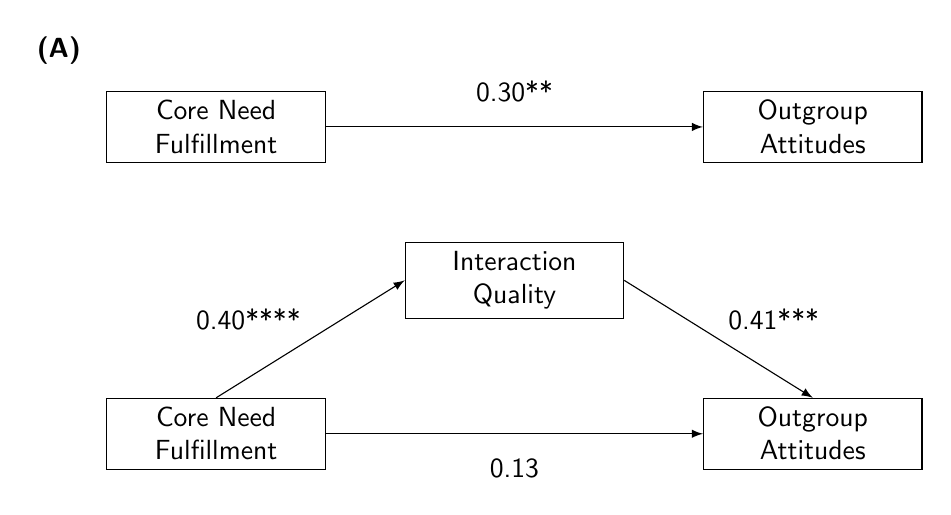
\begin{tikzpicture}[font=\sffamily]
    \node[mynode] (m){Interaction\\Quality};
    \node[mynode,below left=of m](x) {Core Need\\Fulfillment};
    \node[mynode,below right=of m](y) {Outgroup\\Attitudes};
    \node[mynode,above left=of m](xd) {Core Need\\Fulfillment};
    \node[mynode,above right=of m](yd) {Outgroup\\Attitudes};
    \draw[-latex] (xd.east) -- node[above=2mm, align=center] {0.30**} (yd.west);
    \draw[-latex] (x.north) -- node[auto] {0.40****} (m.west);
    \draw[-latex] (m.east) -- node[auto] {0.41***} (y.north);
    \draw[-latex] (x.east) -- node[below=2mm, align=center] {0.13} (y.west);
    \path (xd.north west) ++(-0.2, 6pt) node[above left]{\textbf{(A)}};
\end{tikzpicture}

\vspace{24pt}

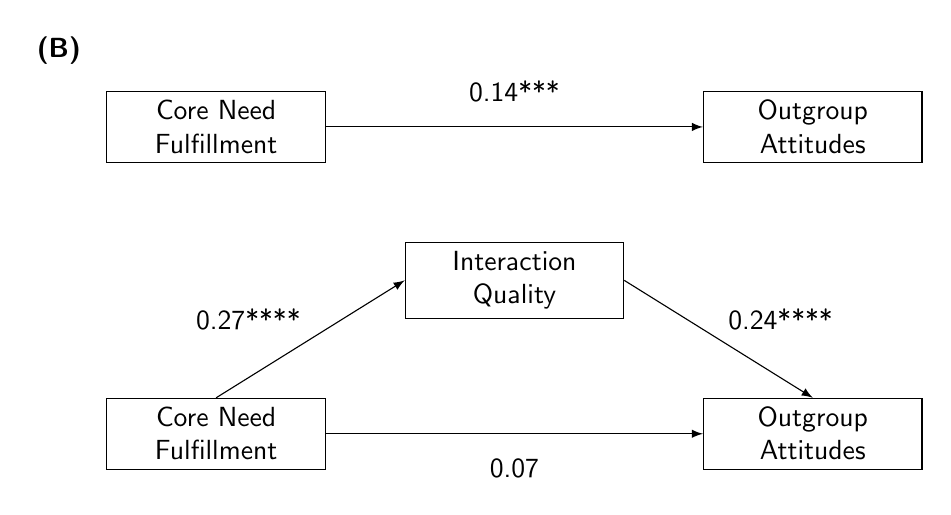
\begin{tikzpicture}[font=\sffamily]
    \node[mynode] (m){Interaction\\Quality};
    \node[mynode,below left=of m](x) {Core Need\\Fulfillment};
    \node[mynode,below right=of m](y) {Outgroup\\Attitudes};
    \node[mynode,above left=of m](xd) {Core Need\\Fulfillment};
    \node[mynode,above right=of m](yd) {Outgroup\\Attitudes};
    \draw[-latex] (xd.east) -- node[above=2mm, align=center] {0.14***} (yd.west);
    \draw[-latex] (x.north) -- node[auto] {0.27****} (m.west);
    \draw[-latex] (m.east) -- node[auto] {0.24****} (y.north);
    \draw[-latex] (x.east) -- node[below=2mm, align=center] {0.07} (y.west);
    \path (xd.north west) ++(-0.2, 6pt) node[above left]{\textbf{(B)}};
\end{tikzpicture}

\vspace{24pt}

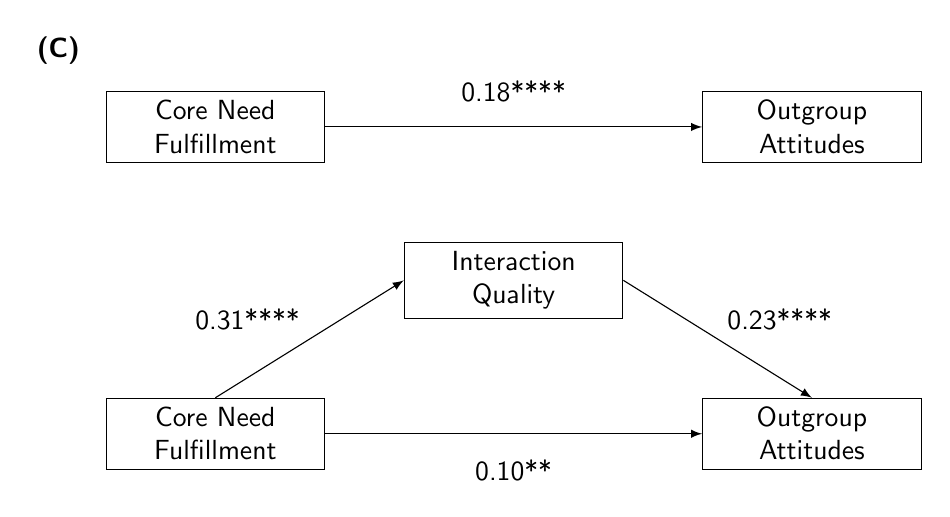
\begin{tikzpicture}[font=\sffamily]
    \node[mynode] (m){Interaction\\Quality};
    \node[mynode,below left=of m](x) {Core Need\\Fulfillment};
    \node[mynode,below right=of m](y) {Outgroup\\Attitudes};
    \node[mynode,above left=of m](xd) {Core Need\\Fulfillment};
    \node[mynode,above right=of m](yd) {Outgroup\\Attitudes};
    \draw[-latex] (xd.east) -- node[above=2mm, align=center] {0.18****} (yd.west);
    \draw[-latex] (x.north) -- node[auto] {0.31****} (m.west);
    \draw[-latex] (m.east) -- node[auto] {0.23****} (y.north);
    \draw[-latex] (x.east) -- node[below=2mm, align=center] {0.10**} (y.west);
    \path (xd.north west) ++(-0.2, 6pt) node[above left]{\textbf{(C)}};
\end{tikzpicture}

  \end{center}
  \caption*{Note: Coefficients are standardized (partial) regression coefficients. Statistical significance markers are based on the unstandardized regression results (as presented in \tblref{tab:intergroupNeedsTblLong}). Note that we do not test a mediation model. The diagram only illustrates the included concepts and partial regression parameters.\\
  **** p < .0001, *** p < .001, ** p < .01, * p < .05}
\end{figure}

\begin{figure}
  \caption{Contact Hypothesis}
  \label{fig:ContactHypothesis}
  \centering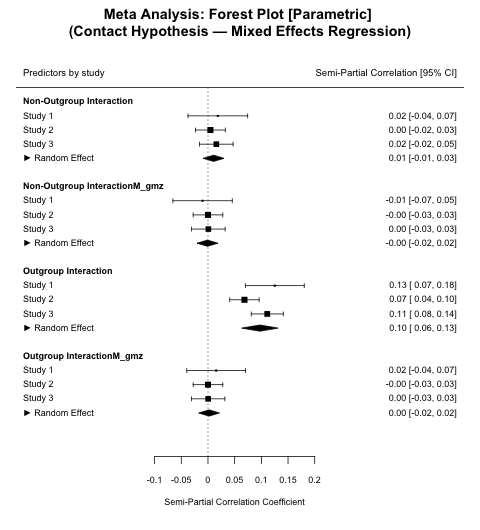
\includegraphics[width=\textwidth]{Figures/forestParametricREMLGeneralLmer.png}
  %\begin{subfigure}{\textwidth}
  %  \caption{}
  %  \centering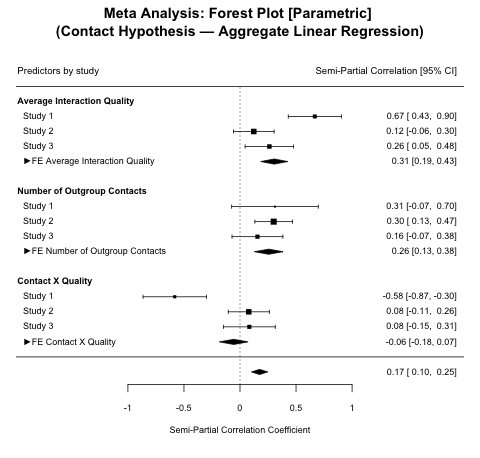
\includegraphics[width=0.75\textwidth]{Figures/forestParametricGeneralLm.png}
  %\end{subfigure}
  %\begin{subfigure}{\textwidth}
  %  \caption{}
  %  \centering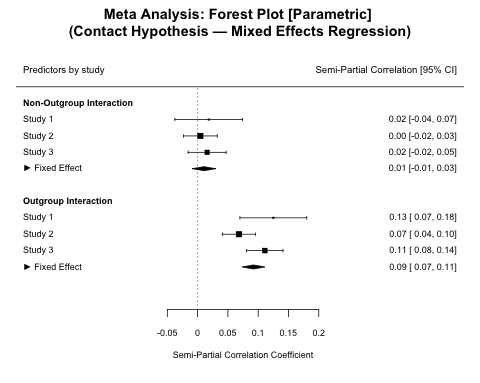
\includegraphics[width=0.75\textwidth]{Figures/forestParametricFEGeneralLmer.png}
  %\end{subfigure}
  \caption*{Note: \\
  Summary of mixed models results of the contemporaneous contact effects.\\
  General: Random effects meta-analytic results are presented for completeness.}
\end{figure}

\begin{figure}
  \caption{Core Need Fulfillment}
  \label{fig:AllportNeedFulfillment}
  \centering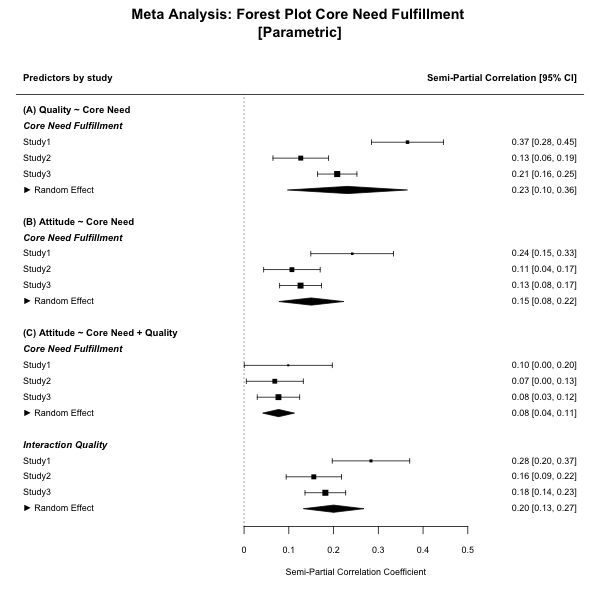
\includegraphics[width=\textwidth]{Figures/forestParametricTheoryComb.png}
  %\begin{subfigure}{\textwidth}
  %  \caption{}
  %  \centering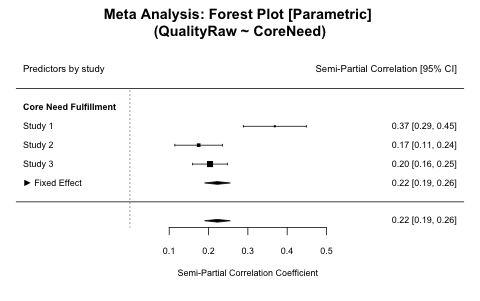
\includegraphics[width=0.6\textwidth]{Figures/forestParametricFETheoryQualityCore.png}
  %\end{subfigure}
  %\begin{subfigure}{\textwidth}
  %  \caption{}
  %  \centering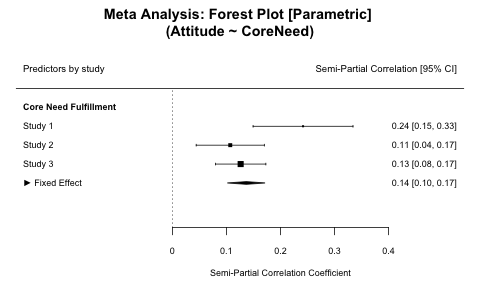
\includegraphics[width=0.6\textwidth]{Figures/forestParametricFETheoryAttitudeCore.png}
  %\end{subfigure}
  %\begin{subfigure}{\textwidth}
  %  \caption{}
  %  \centering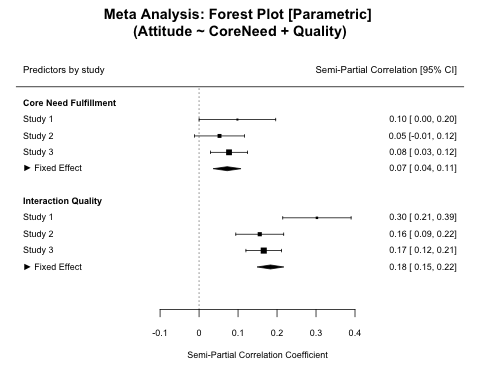
\includegraphics[width=0.6\textwidth]{Figures/forestParametricFETheoryAttitudeCoreQuality.png}
  %\end{subfigure}
  \caption*{Note: \\
  (a) Core Need Fulfillment predicting Interaction Quality.\\
  (b) Core Need Fulfillment predicting Outgroup Attitudes.\\
  (c) Core Need Fulfillment and Interaction Quality predicting Outgroup Attitudes.\\
  General: Random effects meta-analytic results are presented for completeness.}
\end{figure}


\printbibliography

\appendix

\section{Hypotheses and Analysis Plan}
\label{app:AppendixHypotheses}

\newlength{\mdfmar}
\setlength{\mdfmar}{1.5em}
\mdfdefinestyle{mdfhypothesis}{
    innerleftmargin = +1.5\mdfmar, %
    innerrightmargin = +1.5\mdfmar, 
    innertopmargin = +\mdfmar, 
    innerbottommargin = +\mdfmar, 
    skipabove = 12pt
}
\newlength{\subhypskip}
\setlength{\subhypskip}{1.5em}
\newlength{\eqskip}
\setlength{\eqskip}{3.5em}

In this appendix, we present the expanded hypotheses and their associated analysis plan. Given the nested structure of much of our data, we test many of our hypotheses using a multilevel approach, where $y_{ti}$ denotes the response at measurement occasion $t$ ($t = 1, ..., T_i$; level 1) for individual $i$ ($i = 1, ..., n$; level 2). All multilevel assumptions are tested as follows (e.g., for random slopes model with $j$ within-person predictors):

\begin{flalign}
  &\textrm{Level 1 Variance:}\ e_{ti} \sim \mathcal{N}(0,\sigma^2) \\
  &\textrm{Level 2 Variance:}\ \begin{bmatrix} u_{0i}\\ \vdots\\ u_{ji}\end{bmatrix} 
  \sim \mathcal{N}
  \begin{pmatrix}
    \begin{bmatrix} 
      0 \\ 
      \vdots \\
      0
    \end{bmatrix}, 
    \begin{bmatrix} 
      \tau_{00}^2 &  & \\ 
      \vdots & \ddots & \\
      \tau_{j0} & \ldots & \tau_{jj}^2
    \end{bmatrix}
  \end{pmatrix}
\end{flalign}

For our main aims we sequentially focus on four sets of models to test and validate our hypotheses:

\subsection{1. Contact hypothesis in extensive longitudinal data.} 
Within the individual studies, we begin by testing the most basic assumption of the intergroup contact hypothesis that outgroup attitudes should be more positive after outgroup interactions but not after non-outgroup interactions. For this we use multilevel regression analyses, predicting outgroup attitudes from outgroup interaction and non-outgroup interaction dummy variables. We also include the participant means as level two predictors to fully disentangle within- (level 1) and between-participant (level 2) effects of intergroup contact \citep[e.g.,][Section 4.6]{snijders2012}.

\begin{mdframed}[style=mdfhypothesis]
    \begin{hyp}[H\ref{hyp:contactHyp}] \label{hyp:contactHyp}
        Based on the most general understanding of the contact hypothesis, positive intergroup contacts should be associated with more favorable outgroup attitudes across extensive longitudinal data.
    \end{hyp}
    
    \begin{subhyp}[H\ref{hyp:contactDummyML}] \label{hyp:contactDummyML}
    \addtolength{\leftskip}{\subhypskip}
    Outgroup attitudes should be more positive after an intergroup interaction compared to a non-outgroup interaction.
    \end{subhyp}

    \begin{fleqn}[\eqskip] 
    \begin{equation} \label{eq:ContactDummy}
      \begin{split}
        \textrm{Level 1:} &
          \begin{aligned}[t]
            \ Attitude_{ti} =  &\ \beta_{0i} + \beta_{1i}OutgroupInteraction_{ti} + \\
                               &\ \beta_{2i}NonOutgroupInteraction_{ti} + e_{ti}
          \end{aligned} \\
        \textrm{Level 2:} &
            \begin{aligned}[t]
                \ \beta_{0i} = &\ \gamma_{00} + \gamma_{01}MeanOutgroupInteraction_{i} + \\
                               &\ \gamma_{02}MeanNonOutgroupInteraction_{i} + u_{0i} \\
                  \beta_{1i} = &\ \gamma_{10} + u_{1i} \\
                  \beta_{2i} = &\ \gamma_{20} + u_{2i}
            \end{aligned}
      \end{split} 
    \end{equation}
    \end{fleqn}
\end{mdframed}

% We then seek to investigate intergroup contacts and perceived interaction quality jointly. Notably, however, participants are only able to report their interaction quality perceptions if they had an interaction. This is considered to be structurally missing data and cannot meaningfully be imputed for modeling. To deal with this issue, we mimic the procedure commonly used within the cross-section literature. In particular, we conduct a person-level linear regression by aggregating the number of outgroup interactions participants had, their average interaction quality perceptions, as well as their average outgroup attitudes \citep[for possible alternative approaches see,][]{Enders2011}. To avoid an underpowered analysis, we use the aggregated data from all three studies. 
    
We then seek to test the full contact hypothesis by investigating intergroup contacts and perceived interaction quality jointly. To do so, we conduct a linear regression using person-level aggregated data from all three studies. In particular, we aggregate the number of outgroup interactions participants had, their average interaction quality perceptions, as well as their average outgroup attitudes. This approach has three main benefits: (1) Interaction quality ratings are only available if participants had an interaction, and the aggregation deals with this structural missingness. (2) Using the participant-level data from all three studies, we avoid potential power issues. (3) This analysis mimics the analyses conducted within the cross-section literature, where participants are asked to recall how many interactions they had over a one-month period, how positive these interactions were, and what their general attitudes towards the outgroup are.

\begin{mdframed}[style=mdfhypothesis]
    \begin{subhyp}[H\ref{hyp:contactCor}] \label{hyp:contactCor}
    \addtolength{\leftskip}{\subhypskip}
    Participants with more intergroup interactions should have more favorable outgroup attitudes.
    \end{subhyp}

      \begin{fleqn}[\eqskip] 
        \begin{equation} \label{eq:ContactCor}
            r_{\left(ContactFrequency_{i},\ AverageQuality_{i}\right)} > 0
        \end{equation}
      \end{fleqn}

    \begin{subhyp}[H\ref{hyp:contactQualLM}] \label{hyp:contactQualLM}
    \addtolength{\leftskip}{\subhypskip}
    Participants with more intergroup interactions should have more favorable outgroup attitudes depending on the average interaction quality.
    \end{subhyp}

      \begin{fleqn}[\eqskip] 
        \begin{equation} \label{eq:contactQualLM}
            \begin{split}
              AverageAttitude_{i} = &\ \beta_{0} + \beta_{1}ContactFrequency_{i} + \\
                                    &\ \beta_{2}AverageQuality_{i} +\\
                                    &\ \beta_{3}ContactFrequency_{i} * AverageQuality_{i}
            \end{split}
        \end{equation}
      \end{fleqn}  
      
      We additionally control for the participant's study membership.
\end{mdframed}
Because this analysis uses the data from all three studies, the results of this analysis are presented in the `Robustness, Stability, and Embeddedness across Studies' section.

\subsection{2. Core need fulfillment during intergroup contact.}
The main proposal of this manuscript has been the assertion that the fulfillment of situation core needs during an interaction will be associated with more positive interaction quality perceptions and, ultimately, more positive outgroup attitudes. Thus, for the main set of analyses, we focus on the reported outgroup interactions only. For each study, we will use multilevel regressions to test the main three assertions of our proposal (mirroring the basic steps of a traditional mediation analysis).

\begin{mdframed}[style=mdfhypothesis]
    \begin{hyp}[H\ref{hyp:keyNeed}] \label{hyp:keyNeed}
    Based on our proposal, intergroup interactions with higher situational core need fulfillment should predict more favorable outgroup attitudes due to more positive interaction quality perceptions.
    \end{hyp}
    
    \setcounter{subhyp}{0}
    \begin{subhyp}[H\ref{hyp:keyNeedPred}] \label{hyp:keyNeedPred}
    \addtolength{\leftskip}{\subhypskip}
    Core need fulfillment during outgroup interactions should predict more positive outgroup attitudes.
    \end{subhyp}
    
    \begin{fleqn}[\eqskip]
      \begin{equation} \label{eq:SlopesAttCore}
        \begin{split}
            \textrm{Level 1:} &\ Attitude_{ti} = \beta_{0i} + \beta_{1i}KeyNeedFulfill_{ti} + e_{ti}\\
            \textrm{Level 2:} &\ \beta_{0i} = \gamma_{00} + u_{0i} \\
                              &\ \beta_{1i} = \gamma_{10} + u_{1i}
        \end{split}
      \end{equation}
    \end{fleqn}
    
    \begin{subhyp}[H\ref{hyp:keyNeedQual}] \label{hyp:keyNeedQual}
    \addtolength{\leftskip}{\subhypskip}
    Core need fulfillment during outgroup interactions should also predict higher perceived interaction quality.
    \end{subhyp}
    
    \begin{fleqn}[\eqskip]
      \begin{equation} \label{eq:SlopesQltCore}
        \begin{split}
            \textrm{Level 1:} &\ InteractionQuality_{ti} = \beta_{0i} + \beta_{1i}KeyNeedFulfill_{ti} + e_{ti}\\
            \textrm{Level 2:} &\ \beta_{0i} = \gamma_{00} + u_{0i} \\
                              &\ \beta_{1i} = \gamma_{10} + u_{1i}
        \end{split}
      \end{equation}
    \end{fleqn}
    
    \begin{subhyp}[H\ref{hyp:keyNeedMediation}] \label{hyp:keyNeedMediation}
    \addtolength{\leftskip}{\subhypskip}
    The effect of core need fulfillment on outgroup attitudes should be reduced when considered together with perceived interaction quality.
    \end{subhyp}
    
    \begin{fleqn}[\eqskip]
      \begin{equation} \label{eq:SlopesAttCoreQual}
        \begin{split}
          \textrm{Level 1:} &
            \begin{aligned}[t]
              \ Attitude_{ti} =  &\ \beta_{0i} + \beta_{1i}KeyNeedFulfill_{ti} + \\
                                 &\ \beta_{2i}InteractionQuality_{ti} + e_{ti}
            \end{aligned} \\
          \textrm{Level 2:} &\ \beta_{0i} = \gamma_{00} + u_{0i} \\
                            &\ \beta_{1i} = \gamma_{10} + u_{1i} \\
                            &\ \beta_{2i} = \gamma_{20} + u_{2i}
        \end{split} 
      \end{equation}
    \end{fleqn}
\end{mdframed}

\subsection{3. Allport's conditions in extensive longitudinal data.}
Within the third study, we formally measure all of Allport's optimal contact conditions. We use multilevel regression models to test whether the fulfillment of Allport's conditions in real-life data predicts more positive outgroup attitudes and higher perceived interaction quality, using the same approach as for the core need fulfillment above.

\begin{mdframed}[style=mdfhypothesis]
    \begin{hyp}[H\ref{hyp:Allport}] \label{hyp:Allport}
    Based on Allport's optimal contact conditions, intergroup interactions with equal status, common goals, collaboration, and structural support should predict more favorable outgroup attitudes due to more positive interaction quality perceptions.
    \end{hyp}
    
    \setcounter{subhyp}{0}
    \begin{subhyp}[H\ref{hyp:AttAllport}] \label{hyp:AttAllport}
    \addtolength{\leftskip}{\subhypskip}
    Higher fulfillment of Allport's conditions during outgroup interactions should predict more positive outgroup attitudes.
    \end{subhyp}
    
    \begin{fleqn}[\eqskip]
      \begin{equation} \label{eq:SlopesAttAllport}
        \begin{split}
            \textrm{Level 1:} &\ Attitude_{ti} = \beta_{0i} + \beta_{1i}Allport_{ti} + e_{ti}\\
            \textrm{Level 2:} &\ \beta_{0i} = \gamma_{00} + u_{0i} \\
                              &\ \beta_{1i} = \gamma_{10} + u_{1i}
        \end{split}
      \end{equation}
    \end{fleqn}
    
    \begin{subhyp}[H\ref{hyp:QltAllport}] \label{hyp:QltAllport}
    \addtolength{\leftskip}{\subhypskip}
    Higher fulfillment of Allport's conditions during outgroup interactions should also predict higher perceived interaction quality.
    \end{subhyp}
    
    \begin{fleqn}[\eqskip]
      \begin{equation} \label{eq:SlopesQltAllport}
        \begin{split}
            \textrm{Level 1:} &\ InteractionQuality_{ti} = \beta_{0i} + \beta_{1i}Allport_{ti} + e_{ti}\\
            \textrm{Level 2:} &\ \beta_{0i} = \gamma_{00} + u_{0i} \\
                              &\ \beta_{1i} = \gamma_{10} + u_{1i}
        \end{split}
      \end{equation}
    \end{fleqn}
    
    \begin{subhyp}[H\ref{hyp:AttAllportQual}] \label{hyp:AttAllportQual}
    \addtolength{\leftskip}{\subhypskip}
    The effect of higher fulfillment of Allport's conditions on outgroup attitudes should be reduced when considered together with perceived interaction quality.
    \end{subhyp}
    
    \begin{fleqn}[\eqskip]
      \begin{equation} \label{eq:SlopesAttAllportQual}
        \begin{split}
          \textrm{Level 1:} &
            \begin{aligned}[t]
              \ Attitude_{ti} =  &\ \beta_{0i} + \beta_{1i}Allport_{ti} + \\
                                 &\ \beta_{2i}InteractionQuality_{ti} + e_{ti}
            \end{aligned} \\
          \textrm{Level 2:} &\ \beta_{0i} = \gamma_{00} + u_{0i} \\
                            &\ \beta_{1i} = \gamma_{10} + u_{1i} \\
                            &\ \beta_{2i} = \gamma_{20} + u_{2i}
        \end{split} 
      \end{equation}
    \end{fleqn}
\end{mdframed}

We then compare the effect of Allport's contact conditions with our core need fulfillment by comparing the model fit statistics of the two individual models and by adding both concepts to a joint multilevel regression model, to see whether the two approaches explain the same variance in outgroup attitudes.

\begin{mdframed}[style=mdfhypothesis]
    \begin{hyp}[H\ref{hyp:NeedAllport}] \label{hyp:NeedAllport}
    Based on our proposal, the fulfillment of the core situational need should predict outgroup attitudes at least as well as Allport's conditions.
    \end{hyp}

    \setcounter{subhyp}{0}
    \begin{subhyp}[H\ref{hyp:compModel}] \label{hyp:compModel}
    \addtolength{\leftskip}{\subhypskip}
    The need model (H\ref{hyp:keyNeedPred}) should predict more variance in outgroup attitudes than the model based on Allport's conditions (H\ref{hyp:AttAllport}).
    \end{subhyp}

    \begin{fleqn}[\eqskip] 
        \begin{equation}
            \begin{split}
                AIC_{KeyNeedModel} & < AIC_{AllportModel} \\
                BIC_{KeyNeedModel} & < BIC_{AllportModel}
            \end{split}
        \end{equation}
    \end{fleqn}

    \begin{subhyp}[H\ref{hyp:compTogether}] \label{hyp:compTogether}
    \addtolength{\leftskip}{\subhypskip}
    The  effect of key need fulfillment on outgroup attitudes should  persist even when taking other Allport's conditions into account. Thus, the effect of key need fulfillment on outgroup attitudes should remain strong even after controlling for Allport's conditions.  
    \end{subhyp} 
    
    \begin{fleqn}[\eqskip]
      \begin{equation} \label{eq:SlopesAttCoreAllport}
        \begin{split}
          \textrm{Level 1:} &
            \begin{aligned}[t]
              \ Attitude_{ti} =  &\ \beta_{0i} + \beta_{1i}KeyNeedFulfill_{ti} + \\
                                 &\ \beta_{2i}Allport_{ti} + e_{ti}
            \end{aligned} \\
          \textrm{Level 2:} &\ \beta_{0i} = \gamma_{00} + u_{0i} \\
                            &\ \beta_{1i} = \gamma_{10} + u_{1i} \\
                            &\ \beta_{2i} = \gamma_{20} + u_{2i}
        \end{split} 
      \end{equation}
    \end{fleqn}
\end{mdframed}

\subsection{4. Robustness, stability, and embeddedness across studies}
Within the final set of analyses, we look at the broader picture of our results and leverage the data from all participants to contextualize our results.  

\paragraph{Robustness within studies}
To build further confidence in the effect of core need fulfillment during outgroup interactions, we conduct two additional robustness analyses for each study.

Firstly, to check for the role of alternate psychological needs, we add the fulfillment of self-determination theory needs (i.e., competence, autonomy, and relatedness) to the multilevel regression. We then also compare the model with models that predicts outgroup attitudes from self-determination theory need fulfillments or core need fulfillments only. 

\begin{mdframed}[style=mdfhypothesis]
    \begin{hyp}[H\ref{hyp:keyNeedSDT}] \label{hyp:keyNeedSDT}
    The effect of key need fulfillment on outgroup attitudes should persist even when taking other fundamental psychological needs into account. Thus, the effect of key need fulfillment on outgroup attitudes should remain strong even after controlling for autonomy, competence, and relatedness fulfillment during the interaction (cf., self-determination theory). 
    \end{hyp}
    
    \begin{fleqn}[\eqskip-\subhypskip]
      \begin{equation} \label{eq:SlopesAttCoreSdt}
        \begin{split}
          \textrm{Level 1:} &
            \begin{aligned}[t]
              \ Attitude_{ti} =  &\ \beta_{0i} + \beta_{1i}KeyNeedFulfill_{ti} + \beta_{2i}Autonomy_{ti} + \\
                                 &\ \beta_{3i}Competence_{ti} + \beta_{4i}Relatedness_{ti} + e_{ti}
            \end{aligned} \\
          \textrm{Level 2:} &\ \beta_{0i} = \gamma_{00} + u_{0i} \\
                            &\ \beta_{1i} = \gamma_{10} + u_{1i} \\
                            &\ \beta_{2i} = \gamma_{20} + u_{2i} \\
                            &\ \beta_{3i} = \gamma_{30} + u_{3i} \\
                            &\ \beta_{4i} = \gamma_{40} + u_{4i}
        \end{split} 
      \end{equation}
    \end{fleqn}
\end{mdframed}

To ensure that the core need fulfillment is outgroup contact specific, we return to the full sample of intensive longitudinal measurements within each study and test whether there is an interaction effect of outgroup contact (vs. no outgroup contact) and core need fulfillment. We expect that the effect of core need fulfillment is specific to outgroup interactions and not merely due to a more need-fulfilled life in general.

\begin{mdframed}[style=mdfhypothesis]
    \begin{hyp}[H\ref{hyp:keyNeedContactType}] \label{hyp:keyNeedContactType}
    \addtolength{\leftskip}{1em}
    The effect of key need fulfillment on outgroup attitudes should be specific to intergroup interactions and not be due to need fulfillment in general. Thus, the effect of key need fulfillment on outgroup attitudes should be stronger for intergroup interactions than for ingroup interactions. 
    \end{hyp}
    
    \begin{fleqn}[\eqskip-\subhypskip]
      \begin{equation} \label{eq:SlopesAttCoreXContact}
        \begin{split}
          \textrm{Level 1:} &
            \begin{aligned}[t]
              \ Attitude_{ti} =  &\ \beta_{0i} + \beta_{1i}KeyNeedFulfill_{ti} + \\
                                 &\ \beta_{2i}OutgroupInteraction_{ti} + \\
                                 &\ \beta_{3i}KeyNeedFulfill*OutgroupInteraction_{ti} + e_{ti}
            \end{aligned} \\
          \textrm{Level 2:} &\ \beta_{0i} = \gamma_{00} + u_{0i} \\
                            &\ \beta_{1i} = \gamma_{10} + u_{1i} \\
                            &\ \beta_{2i} = \gamma_{20} + u_{2i} \\
                            &\ \beta_{3i} = \gamma_{30} + u_{3i}
        \end{split} 
      \end{equation}
    \end{fleqn}
\end{mdframed}
The results of the robustness analyses are presented in \appref{app:AppendixRobustness} to allow for a more concise presentation of our main hypotheses in the main text.

\paragraph{Stability across studies}
We assess the stability of our main analyses. We use forest plots (including meta-analytical estimates) to visualize the direction and effect sizes of our three studies.

\begin{mdframed}[style=mdfhypothesis]
    \begin{hyp}[H\ref{hyp:Stability}] \label{hyp:Stability}
    \addtolength{\leftskip}{1em}
    The effects of our main hypotheses and robustness analyses should be consistent across studies.
    \end{hyp}
\end{mdframed}

\paragraph{Embeddedness of code needs}
We, finally, use the qualitative data from the participants' self-identified core needs to contextualize our results. We leverage machine learning to extract a topic model of the free-text entries across the three studies. We describe the extracted topics and themes and compare them to the need contents usually found and measured within the psychological literature. Full methodological details and visualizations are available in Supplemental Material B.

\begin{mdframed}[style=mdfhypothesis]
    \addtolength{\leftskip}{1em}
    \textit{This analysis is data-driven and exploratory. As such, the analysis has no associated hypothesis.}
\end{mdframed}



\section{Robustness Analyses}
\label{app:AppendixRobustness}

In this appendix, we present the empirical details of our additional robustness analyses. These analyses are specifically designed to check for alternative models and contextualize our results. We (1) check whether core need fulfillment is indeed outgroup contact specific. For this analysis, we return to the full sample of intensive longitudinal measurements and test whether there is an interaction effect of outgroup contact (vs. no outgroup contact) and core need fulfillment. We expect that the effect of core need fulfillment is specific to outgroup interactions and not merely due to a more need-fulfilled life in general. We then check (2) whether the need mechanism is relevant to both planned and accidental outgroup interactions, and (3) extends to the more individual-focused experience of well-being. In a final set of analyses, we (4) check whether the need fulfillment mechanism is relevant to different types of need content (i.e., motives) and (5) remains relevant even when accounting for the fulfillment of fundamental psychological needs (i.e., self-determination theory needs: competence, autonomy, and relatedness).

As with the main analyses, full surveys are available in our OSF
repository \citep{KreienkampMasked2022a} and the full data description
is available in Online Supplementary Material A. Correlations and
descriptive statistics of the included variables are available in
\tblref{tab:descrFullWide} and \tblref{tab:descrOutWide}.

\subsection{Additional Materials}

In addition to the measurement of whether or not participants had an
intergroup interaction and their situational core need fulfillment, we
also included a number of variables that allowed us to assess the
robustness of our results.

\subsubsection{Specific Psychological Needs}

In addition to the intergroup contact dummy and situational core need
reported in the main text, we included a common measure of three
self-determination theory needs \citep[see][]{Downie2008}. The
measurement was identical in all three studies. The items were
introduced either by ``\textit{During the interaction:}'' or
``\textit{This morning [/afternoon]:}'' and measured autonomy
(``\textit{I was myself.}''), competence
(``\textit{I felt competent.}''), and relatedness (without intergroup
contact ``\textit{I had a strong need to belong}''; with intergroup
contact: ``\textit{I shared information about myself.}'' and
``\textit{The other(s) shared information about themselves.}''). All
items were rated on a continuous slider scale from very little (-50) to
a great deal (+50).

\subsubsection{Interaction Intent}

To assess whether an interaction was accidental (vs.~planned), we asked
participants with a single item to report the extend to which ``The
interaction with -X- was accidental''. The respondents were asked to
report this context variable for all interactions they reported on using
a continuous slider ranging from ``not at all'' (0), through ``very
little'' (33) and ``somewhat'' (66), to ``a great deal'' (100). In all
studies the scale showed a right skew (\textit{mean} = 29.60,
\textit{sd} = 33.68).

\subsubsection{Goal-directedness}

To assess whether the need content (i.e., the motives) would impact the
effect of the need fulfillment experiences, we manually coded the topics
we extracted during the topic modeling on two dimensions of how much
they reflect a practical and a psychological goal-directedness. We chose
practical and psychological needs specifically as our dimensions to
account for differences in the types of needs that participants commonly
reported. With practical motives we refer to specific, tangible goals or
tasks that participants aimed to accomplish during the interaction.
These instrumental goals are usually observable, concrete, and often
centered on external outcomes, such as acquiring resources, completing
tasks, and addressing immediate challenges \citep[e.g.,][]{oduntan2019}.
With psychological motives we refer to underlying motives or desires
that are more abstract and relate to personal fulfillment and
well-being. In contrast to practical needs, psychological needs delve
into the subjective and internal aspects of human experiences. These
needs pertain to emotions, social connections, and cognitive processes,
reflecting individuals' quest for personal growth, well-being, and
thriving in social relationships \citep[][]{dweck2017}. Note that with
this approach any particular motive can include a practical and/or a
psychological goal-directedness but can also be classified as not having
any goal at all. The full coding protocol we developed with examples for
each of the codes is available in our Online Supplemental Material D.
After an initial training, each of the two coders independently coded
the 47 topics on the two dimensions, using one of three options each
(i.e., 0 = no goal, 1 = vague goal, 2 = clear goal). Inter-rater
reliability assessments showed that for both the practical as well as
the psychological needs, agreement was not optimal using the three
answer options (agreement practical = 0.72\%, agreement psychological =
0.78\%). However, most disagreements were, if a need was present,
whether that need was vague (1) or concrete (2). We, thus, collapsed
these two categories making the ratings binary (need absent vs.~need
present). With the simpler coding, inter-rater agreement for practical
needs (0.93\%) and the psychological need (0.96\%) were much more
reliable. Using Cohen's \(\kappa\) as our measure of inter-rater
reliability, we find that both the practical need coding
(\textit{Cohen's} \(\kappa\) = 0.80, 95\%CI{[}0.58, 1.00{]}) as well as
the psychological need coding (\textit{Cohen's} \(\kappa\) = 0.86,
95\%CI{[}0.67, 1.00{]}) were very good. We thus proceeded with this
collapsed coding. After resolving coder disagreements and merging the
codings back to the free-text responses, we found that a majority of
responses showed both a practical as well as a psychological need
(57.95\%) and only few responses had no goal at all (1.03\%) with the
remaining 41.02\% having either a practical or a psychological need only
(see Online Supplemental Material A for more detailed tables and
visualizations).

\subsubsection{Well-being}

We measured experienced well-being using a visual analog scale adapted
from \citet{davies2022}. Participants were asked to respond to the the
question ``How do you feel right now?'' using a continuous visual slider
ranging from ``very sad''(-100) to ``very happy'' (100). The well-being
ratings were generally normally distributed (\textit{mean} = 64.80,
\textit{sd} = 19.25).

\subsection{Results}

To build further confidence in our results, we assessed a number of
additional models that might offer alternative explanations. We will
discuss the results in sequential order --- in every case first
considering the a global test of the model across the three studies and
only then assessing whether the global three-level regression model
suppresses any important person-level variations within the studies.

\subsubsection{Contact specific}

We begin our robustness analysis by testing whether the effect of core
need fulfillment is specific to an actual outgroup contact, rather than
need fulfillment in general. For this, we analyzed the generalized
situational core need fulfillment (either during a contact or about the
daytime in general) and tested whether the effect differed during
experience sampling measurements with and without outgroup contacts. We
start this test by assessing the effect across all three studies, using
a three-level hierarchical model, where measurements are nested within
participants, and participants are nested within studies. In this
overall model, we found no main effect of core need fulfillment (random
slopes model, grand-mean standardized to account for all levels of
variance; \textit{b} = 0.62, \textit{t}( 3.187) = 2.89, \textit{p} =
0.058, \textit{95\%CI}{[} 0.20, 1.03{]}) but a significant interaction
effect of core need fulfillment and outgroup contact (\textit{b} = 2.44,
\textit{t}(4,663.172) = 8.62, \textit{p} \textless{} .001,
\textit{95\%CI}{[} 1.89, 3.00{]}; also see
\tblref{tab:robustnessTblLong}). While the three-level hierarchical
model can be sensitive to scaling issues, this already indicates that it
is not key need fulfillment in general --- but only key need fulfillment
during an outgroup contact that predicts more positive outgroup
attitudes.

To ensure that the results are not affected by scaling issues (e.g.,
study-level variances suppressing person-level variances) or a similar
Simpson's paradox, we additionally assess the model within each of the
three studies. Within each of the three studies, the effects are more
pronounced, so that we also see a significant effect of core need
fulfillment (all \textit{b} \textgreater{} 0.06, all \textit{p}
\textless{} 0.005) as well as outgroup contact itself (all
\textbar{}\textit{b}\textbar{} \textgreater{} 1.81, all \textit{p}
\textless{} 0.034) but the interaction effect consistently remains the
most reliable predictor of outgroup attitudes (all
\textbar{}\textit{b}\textbar{} \textgreater{} 0.06, all \textit{p}
\textless{} 0.002, also see \tblref{tab:robustnessTblLong}). There is
thus consistent evidence that need fulfillment relates to outgroup
attitudes for outgroup contacts in particular but not need fulfillment
in general.

\subsubsection{Interaction intent}

Secondly, to assess whether the need fulfillment mechanism affected by
whether the interaction was accidental or planned we ran an exploratory
moderation analysis using the participants' ratings of how much they
perceived the interaction as `accidental'. It should be noted that we
asked our participants to focus on most the important interaction (i.e.,
``\textit{The following questions will be about the interaction \underline{you consider most significant}.}'';
emphasis as in original). We again start our analysis approach by
assessing the model across all three studies, using a three-level
hierarchical model. In this overall model, we retain the main effect of
core need fulfillment (random slopes model, grand-mean standardized to
account for all levels of variance; \textit{b} = 2.87, \textit{t}(
7.979) = 7.32, \textit{p} \textless{} .001, \textit{95\%CI}{[} 2.10,
3.64{]}) but neither contact intent nor the moderation effect affect the
results (all \textbar{}\textit{b}\textbar{} \textless{} 0.27 and all
\textit{p} \textgreater{} 0.225; see \tblref{tab:robustnessTblLong} for
full results).

We again sought to ensure that the results were not affected by scaling
issues by additionally assessing the interaction intentionality model
within each of the three studies. Within each of the three studies, the
effect of core need fulfillment became even clearer (all
\textbar{}\textit{b}\textbar{} \textgreater{} 0.13, all \textit{p}
\textless{} 0.006). But in none of the studies neither outgroup contact
intention nor the moderation effect explained a significant amount of
variance in outgroup attitudes (all \textbar{}\textit{b}\textbar{}
\textless{} 0.03 and all \textit{p} \textgreater{} 0.073; also see
\tblref{tab:robustnessTblLong}). There is thus consistent evidence that
need fulfillment is related to outgroup attitudes, even when taking the
intentionality of the interaction into account --- at least in our three
samples and with a focus on the most significant interactions.

\subsubsection{Well-being outcome}

Thirdly, to build a stronger case for the relevance of need fulfillment
to minority group members, we exploratorily assessed the effect of need
fulfilling outgroup interactions on self-reported well-being. We, thus,
re-ran our main analysis but substituted the outgroup attitudes outcome
with situational well-being. As with the previous robustness analyses,
we begin with a global three-level hierarchical model (across the three
studies). We find that need fulfillment during outgroup contacts,
indeed, has a similar effect on experienced well-being (random slopes
model, grand-mean standardized to account for all levels of variance;
\textit{b} = 3.50, \textit{t}(4.219) = 6.33, \textit{p} = 0.003,
\textit{95\%CI}{[} 2.42, 4.58{]}). We found the same result when we
assessed each of the three studies individually. In each of the studies
situational need fulfillment during the outgroup interaction was related
with higher well-being ratings by the participants (random slopes model,
centered within participants; all \textbar{}\textit{b}\textbar{}
\textgreater{} 0.10, all \textit{p} \textless{} 0.009). We, thus, find
consistent and meaningful evidence that need fulfilling outgroup
interactions also relate to higher everyday well-being.

\subsubsection{Need types}

Fourthly, to assess the role of different types of motives reported by
our participants, we added our coding of practical and psychological
goal-directedness as additional predictors to our base model. We thus
had core need fulfillment predicting outgroup attitudes while also
accounting for whether the reported motives were capturing practical
and/or psychological motives. We again ran a global model, across the
three studies first. We found that core need fulfillment remain a core
predictor of outgroup attitudes (random slopes model, grand-mean
standardized to account for all levels of variance; \textit{b} = 2.27,
\textit{t}( 48.194) = 2.72, \textit{p} = 0.009, \textit{95\%CI}{[} 0.63,
3.90{]}), even after accounting for different types of motives. None of
the motive types nor the moderation effects reached statistical
significance within the overall analysis (all
\textbar{}\textit{b}\textbar{} \textless{} 1.45 and all \textit{p}
\textgreater{} 0.073; see \tblref{tab:robustnessTblLong} for full
results).

When looking at the individual studies, we again saw that the effect of
core need fulfillment remained the on only clear effect (all
\textbar{}\textit{b}\textbar{} \textgreater{} 0.14, all \textit{p}
\textless{} 0.015). Additionally, in none of the studies neither motive
type dummies nor the moderation effect explained a significant amount of
variance in outgroup attitudes (all \textbar{}\textit{b}\textbar{}
\textless{} 1.53 and all \textit{p} \textgreater{} 0.144; also see
\tblref{tab:robustnessTblLong}). We, thus, find consistent evidence that
need fulfillment is related to outgroup attitudes, even when taking the
type of need into account --- at least in our three samples.

\subsubsection{Specific psychological needs}

In a final step, we checked whether during the interaction the core
situational need remains a meaningful predictor even when taking other
fundamental psychological needs into account. We again take a two-step
approach, starting with cross-study global three-level test and then
assessing the effects within the individual studies. Within the overall
model we find that across the studies core need fulfillment remained a
strong predictor of outgroup attitudes, even after controlling for the
three self-determination theory need (random slopes model, grand-mean
standardized to account for all levels of variance; \textit{b} = 1.88,
\textit{t}(2.702) = 4.75, \textit{p} = 0.022, \textit{95\%CI}{[} 1.11,
2.66{]}). Within this overall analysis, none of the self-determination
theory needs independently predicted outgroup attitudes to a
statistically significant extent (all \textit{p} \textgreater{} 0.093).
However, some of the effect sizes were largely comparable to that of the
core need fulfillment (all \textbar{}\textit{b}\textbar{} \textless{}
2.10, particularly that of relatedness fulfillment; see
\tblref{tab:robustnessTblLong} for full results).

When looking at the individual studies, we again saw that core need
fulfillment remained a consistent predictor of outgroup attitudes, even
after accounting for the self-determination theory need (all
\textbar{}\textit{b}\textbar{} \textgreater{} 0.06, all \textit{p}
\textless{} 0.030). However, across all three studies the fulfillment of
relatedness motives also emerged as a consistent predictor of outgroup
attitudes (all \textbar{}\textit{b}\textbar{} \textgreater{} 0.06, all
\textit{p} \textless{} 0.001). Additionally, in the larger studies 2 and
3 competence fulfillment was also related to more positive outgroup
attitudes (study 2: \textit{b} = 0.05, \textit{t}(841.8) = 2.43,
\textit{p} = 0.015, \textit{95\%CI}{[} 0.01, 0.10{]}, study 3:
\textit{b} = 0.06, \textit{t}(30.20) = 2.62, \textit{p} = 0.013,
\textit{95\%CI}{[} 0.01, 0.10{]}). None of the autonomy fulfillment
effects reached statistical significance nor did the competence
fulfillment during study 1 (see \tblref{tab:robustnessTblLong} for the
full results). In short, find that across our samples, relatedness
fulfillment (and to a smaller extend competence fulfillment) are
instrumental in understanding when an outgroup contact leads to more
positive outgroup attitudes. Importantly, even when considering these
effects situational core need fulfillment remains a strong and
consistent predictor of outgroup attitudes. In some cases, we even find
that core need fulfillment takes on some of the variance that would
otherwise be explained by the self-determination theory needs (see
Online Supplemental Material A).



% Tables
\begin{table}
\begin{minipage}[t][\textheight][t]{\textwidth}

\caption{\label{tab:descrFullWideAppB}Full Sample: Correlation Table and Descriptive Statistics}
\centering
\resizebox{\linewidth}{!}{
\begin{tabular}[t]{lccccccccccccc}
\toprule
\multicolumn{1}{c}{} & \multicolumn{8}{c}{Correlations} & \multicolumn{5}{c}{Descriptives} \\
\cmidrule(l{3pt}r{3pt}){2-9} \cmidrule(l{3pt}r{3pt}){10-14}
Variable & Core Need & Competence & Autonomy & Relatednesss & Outgroup Interaction & Accidental & Quality & Attitudes NL & Grand Mean & Between SD & Within SD & ICC(1) & ICC(2)\\
\midrule
\addlinespace[0.3em]
\multicolumn{14}{l}{\textbf{Study 1}}\\
\hspace{1em}Core Need &  & 0.36*** & 0.31*** & 0.45*** & 0.05 &  &  & 0.10*** & 77.95 & 14.68 & 20.83 & 0.29 & 0.96\\
\hspace{1em}Competence & 0.61*** &  & 0.08** & 0.15*** & 0.10*** &  &  & 0.00 & 62.10 & 13.72 & 20.89 & 0.28 & 0.95\\
\hspace{1em}Autonomy & 0.46** & 0.71*** &  & -0.02 & 0.11*** &  &  & 0.14*** & 72.17 & 12.09 & 15.15 & 0.38 & 0.97\\
\hspace{1em}Relatednesss & -0.01 & -0.11 & -0.04 &  & 0.12*** &  &  & 0.14*** & 55.29 & 14.59 & 23.29 & 0.28 & 0.95\\
\hspace{1em}Outgroup Interaction & 0.24 & 0.45* & 0.24 & 0.15 &  &  &  & 0.13*** & -1.71 & 0.21 & 0.41 & 0.17 & 0.91\\
\hspace{1em}Attitudes NL & -0.20 & -0.21 & 0.21 & -0.06 & 0.11 &  &  &  & 71.49 & 12.91 & 8.11 & 0.70 & 0.99\\
\addlinespace[0.3em]
\multicolumn{14}{l}{\textbf{Study 2}}\\
\hspace{1em}Core Need &  & 0.24*** & 0.15*** & 0.45*** & 0.16*** & 0.35*** & 0.34*** & -0.05** & 84.87 & 9.17 & 20.33 & 0.15 & 0.89\\
\hspace{1em}Competence & 0.56*** &  & -0.12*** & -0.18*** & -0.29*** & -0.11*** & -0.04* & -0.11*** & 72.55 & 14.47 & 21.17 & 0.30 & 0.95\\
\hspace{1em}Autonomy & 0.62*** & 0.70*** &  & -0.09*** & 0.15*** & 0.21*** & 0.36*** & 0.42*** & 82.59 & 11.21 & 16.06 & 0.32 & 0.95\\
\hspace{1em}Relatednesss & 0.37*** & 0.64*** & 0.53*** &  & 0.52*** & -0.21*** & -0.25*** & 0.08*** & 61.21 & 13.36 & 28.74 & 0.17 & 0.90\\
\hspace{1em}Outgroup Interaction & -0.20 & -0.20* & -0.15 & -0.35*** &  & 0.11*** & 0.05** & 0.11*** & -1.80 & 0.17 & 0.36 & 0.16 & 0.90\\
\hspace{1em}Accidental & -0.49*** & -0.22* & -0.33*** & -0.10 & 0.13 &  & 0.11*** & 0.03 & 25.09 & 14.62 & 29.13 & 0.17 & 0.85\\
\hspace{1em}Quality & 0.54*** & 0.69*** & 0.60*** & 0.62*** & -0.23* & -0.33*** &  & 0.09*** & 74.51 & 11.24 & 16.59 & 0.29 & 0.92\\
\hspace{1em}Attitudes NL & 0.11 & 0.06 & -0.06 & -0.12 & 0.33*** & 0.03 & 0.11 &  & 67.26 & 18.64 & 9.40 & 0.80 & 0.99\\
\addlinespace[0.3em]
\multicolumn{14}{l}{\textbf{Study 3}}\\
\hspace{1em}Core Need &  & 0.27*** & 0.31*** & 0.55*** & 0.20*** & 0.39*** & 0.51*** & -0.09*** & 83.57 & 8.02 & 17.14 & 0.18 & 0.92\\
\hspace{1em}Competence & 0.49*** &  & -0.21*** & -0.30*** & -0.40*** & -0.10*** & -0.14*** & -0.16*** & 77.45 & 11.49 & 18.92 & 0.26 & 0.95\\
\hspace{1em}Autonomy & 0.58*** & 0.78*** &  & -0.13*** & 0.15*** & 0.37*** & 0.38*** & 0.54*** & 83.76 & 9.72 & 15.87 & 0.28 & 0.96\\
\hspace{1em}Relatednesss & 0.22 & 0.49*** & 0.46*** &  & 0.50*** & -0.25*** & -0.21*** & 0.10*** & 63.44 & 13.34 & 28.85 & 0.17 & 0.92\\
\hspace{1em}Outgroup Interaction & 0.04 & -0.16 & -0.15 & 0.06 &  & 0.06** & 0.01 & -0.04* & -1.57 & 0.20 & 0.46 & 0.15 & 0.91\\
\hspace{1em}Accidental & -0.50*** & -0.23* & -0.27* & -0.04 & -0.08 &  & 0.24*** & 0.02 & 24.73 & 14.98 & 28.51 & 0.21 & 0.92\\
\hspace{1em}Quality & 0.40*** & 0.55*** & 0.60*** & 0.52*** & -0.12 & -0.02 &  & 0.08*** & 76.62 & 12.42 & 16.98 & 0.34 & 0.96\\
\hspace{1em}Attitudes NL & 0.11 & 0.12 & 0.11 & 0.20 & 0.22 & 0.02 & 0.11 &  & 64.77 & 14.37 & 10.88 & 0.66 & 0.99\\
\addlinespace[0.3em]
\multicolumn{14}{l}{\textbf{Across Studies}}\\
\hspace{1em}Core Need &  & 0.31*** & 0.28*** & 0.55*** & 0.21*** & 0.41*** & 0.44*** & -0.10*** & 83.81 & 7.85 & 20.24 & 0.11 & 0.92\\
\hspace{1em}Competence & 0.50*** &  & -0.19*** & -0.26*** & -0.35*** & -0.14*** & -0.11*** & -0.14*** & 73.38 & 11.52 & 22.25 & 0.18 & 0.95\\
\hspace{1em}Autonomy & 0.57*** & 0.71*** &  & -0.11*** & 0.13*** & 0.32*** & 0.43*** & 0.50*** & 82.36 & 9.35 & 16.98 & 0.21 & 0.96\\
\hspace{1em}Relatednesss & 0.24* & 0.55*** & 0.48*** &  & 0.52*** & -0.21*** & -0.22*** & 0.15*** & 61.55 & 10.73 & 29.45 & 0.11 & 0.91\\
\hspace{1em}Outgroup Interaction & -0.21* & -0.11 & -0.08 & -0.18 &  & 0.11*** & 0.08*** & 0.08*** & -1.73 & 0.17 & 0.42 & 0.11 & 0.92\\
\hspace{1em}Accidental & -0.50*** & -0.22* & -0.37*** & -0.01 & 0.10 &  & 0.13*** & -0.01 & 24.56 & 12.38 & 29.70 & 0.12 & 0.89\\
\hspace{1em}Quality & 0.39*** & 0.58*** & 0.55*** & 0.54*** & -0.13 & -0.11 &  & 0.17*** & 75.46 & 9.44 & 17.85 & 0.19 & 0.93\\
\hspace{1em}Attitudes NL & -0.03 & 0.05 & -0.05 & -0.13 & 0.33*** & 0.08 & 0.01 &  & 66.58 & 14.46 & 13.25 & 0.49 & 0.99\\
\bottomrule
\multicolumn{14}{l}{\rule{0pt}{1em}\textit{Note: }}\\
\multicolumn{14}{l}{\rule{0pt}{1em}Upper triangle: Between-person correlations;}\\
\multicolumn{14}{l}{\rule{0pt}{1em}Lower triangle: Within-person correlations;}\\
\multicolumn{14}{l}{\rule{0pt}{1em}*** p < .001, ** p < .01,  * p < .05}\\
\multicolumn{14}{l}{\rule{0pt}{1em}Interaction Intent and Interaction Quality were only measured for outgroup interactions in Study 1.}\\
\end{tabular}}
\end{minipage}
\end{table}

\begin{table}
\begin{minipage}[t][\textheight][t]{\textwidth}

\caption{\label{tab:descrOutWideAppB}Outgroup Interaction Sample: Correlation Table and Descriptive Statistics}
\centering
\resizebox{\linewidth}{!}{
\begin{tabular}[t]{lcccccccccccccc}
\toprule
\multicolumn{1}{c}{} & \multicolumn{9}{c}{Correlations} & \multicolumn{5}{c}{Descriptives} \\
\cmidrule(l{3pt}r{3pt}){2-10} \cmidrule(l{3pt}r{3pt}){11-15}
Variable & Core Need & Competence & Autonomy & Relatednesss & Practical Need & Psychological Need & Accidental & Quality & Attitudes NL & Grand Mean & Between SD & Within SD & ICC(1) & ICC(2)\\
\midrule
\addlinespace[0.3em]
\multicolumn{15}{l}{\textbf{Study 1}}\\
\hspace{1em}Core Need &  & 0.32*** & 0.26*** & 0.48*** & 0.17** & 0.21*** & 0.21*** & -0.03 & -0.09 & 82.20 & 12.42 & 17.66 & 0.33 & 0.90\\
\hspace{1em}Competence & 0.83*** &  & -0.11* & -0.08 & -0.09 & -0.06 & 0.08 & 0.12* & -0.20*** & 66.53 & 13.41 & 18.78 & 0.31 & 0.89\\
\hspace{1em}Autonomy & 0.65*** & 0.85*** &  & -0.10 & -0.04 & -0.01 & 0.18** & -0.17** & 0.15** & 72.64 & 10.22 & 14.93 & 0.30 & 0.89\\
\hspace{1em}Relatednesss & 0.25 & 0.25 & 0.27 &  & 0.34*** & 0.41*** & 0.36*** & 0.47*** & -0.08 & 51.58 & 14.16 & 23.97 & 0.21 & 0.83\\
\hspace{1em}Practical Need & 0.37 & 0.36 & 0.17 & -0.17 &  & 0.13* & -0.12* & 0.16** & 0.18*** & 0.20 & 0.19 & 0.43 & 0.10 & 0.65\\
\hspace{1em}Psychological Need & -0.41 & -0.18 & -0.16 & 0.42** & -0.60** &  & 0.21*** & 0.38*** & 0.00 & 0.28 & 0.19 & 0.38 & 0.13 & 0.70\\
\hspace{1em}Accidental & 0.15 & 0.12 & 0.11 & -0.23 & 0.21 & -0.44 &  & 0.04 & 0.08 & 28.49 & 20.85 & 27.58 & 0.30 & 0.89\\
\hspace{1em}Quality & 0.46* & 0.44* & 0.41 & 0.35 & 0.23 & 0.15 & 0.11 &  & 0.55*** & 67.00 & 9.26 & 18.24 & 0.23 & 0.84\\
\hspace{1em}Attitudes NL & 0.05 & -0.22 & 0.08 & 0.07 & -0.31 & 0.11 & 0.27 & 0.21 &  & 72.46 & 13.62 & 9.50 & 0.68 & 0.98\\
\addlinespace[0.3em]
\multicolumn{15}{l}{\textbf{Study 2}}\\
\hspace{1em}Core Need &  & 0.22*** & 0.10** & 0.50*** & 0.18*** & 0.32*** & 0.24*** & 0.01 & 0.00 & 86.91 & 11.16 & 15.92 & 0.13 & 0.57\\
\hspace{1em}Competence & 0.48** &  & -0.08* & -0.26*** & 0.07* & 0.06 & 0.04 & 0.17*** & -0.17*** & 73.26 & 13.96 & 16.80 & 0.27 & 0.76\\
\hspace{1em}Autonomy & 0.54*** & 0.60*** &  & -0.13*** & -0.02 & 0.03 & 0.11** & -0.16*** & -0.01 & 78.58 & 14.07 & 14.23 & 0.40 & 0.85\\
\hspace{1em}Relatednesss & -0.13 & 0.53*** & 0.27* &  & 0.20*** & 0.40*** & 0.37*** & 0.47*** & -0.08* & 60.32 & 17.38 & 26.14 & 0.19 & 0.66\\
\hspace{1em}Practical Need & 0.16 & -0.24 & -0.10 & -0.39** &  & 0.13*** & -0.16*** & 0.16*** & 0.21*** & 0.23 & 0.29 & 0.38 & 0.15 & 0.57\\
\hspace{1em}Psychological Need & 0.24 & 0.09 & -0.02 & 0.27 & -0.33 &  & 0.15*** & 0.22*** & 0.03 & 0.30 & 0.24 & 0.37 & 0.12 & 0.51\\
\hspace{1em}Accidental & -0.63*** & -0.11 & -0.26* & 0.16 & 0.03 & -0.10 &  & 0.07 & -0.01 & 33.53 & 23.45 & 29.73 & 0.28 & 0.77\\
\hspace{1em}Quality & 0.36* & 0.49*** & 0.51*** & 0.54*** & -0.16 & 0.07 & -0.23 &  & 0.28*** & 67.10 & 12.55 & 16.53 & 0.24 & 0.73\\
\hspace{1em}Attitudes NL & 0.18 & 0.28* & 0.13 & -0.11 & 0.05 & 0.10 & -0.06 & 0.05 &  & 70.41 & 17.13 & 9.86 & 0.72 & 0.96\\
\addlinespace[0.3em]
\multicolumn{15}{l}{\textbf{Study 3}}\\
\hspace{1em}Core Need &  & 0.24*** & 0.25*** & 0.50*** & 0.14*** & 0.31*** & 0.43*** & 0.04 & -0.02 & 84.84 & 9.25 & 13.00 & 0.30 & 0.91\\
\hspace{1em}Competence & 0.56*** &  & -0.07** & -0.27*** & -0.06* & -0.05 & -0.01 & 0.05 & -0.26*** & 75.91 & 12.27 & 17.20 & 0.29 & 0.91\\
\hspace{1em}Autonomy & 0.59*** & 0.78*** &  & -0.06* & -0.09*** & -0.06* & -0.01 & -0.15*** & -0.02 & 79.12 & 12.86 & 15.26 & 0.36 & 0.93\\
\hspace{1em}Relatednesss & 0.15 & 0.44*** & 0.45*** &  & 0.33*** & 0.30*** & 0.43*** & 0.41*** & -0.07** & 59.69 & 19.27 & 23.46 & 0.34 & 0.93\\
\hspace{1em}Practical Need & -0.24 & -0.30* & -0.25 & -0.52*** &  & 0.04 & -0.16*** & 0.21*** & 0.21*** & 0.27 & 0.20 & 0.39 & 0.14 & 0.76\\
\hspace{1em}Psychological Need & 0.05 & -0.09 & -0.09 & -0.14 & -0.07 &  & 0.19*** & 0.19*** & -0.03 & 0.35 & 0.16 & 0.33 & 0.13 & 0.75\\
\hspace{1em}Accidental & -0.37** & -0.16 & -0.18 & 0.11 & -0.19 & -0.21 &  & 0.04 & -0.04 & 29.22 & 17.93 & 30.40 & 0.25 & 0.89\\
\hspace{1em}Quality & 0.48*** & 0.59*** & 0.65*** & 0.52*** & -0.52*** & -0.12 & -0.01 &  & 0.29*** & 71.95 & 14.98 & 16.72 & 0.43 & 0.95\\
\hspace{1em}Attitudes NL & 0.25 & 0.32** & 0.34** & 0.40*** & -0.05 & -0.16 & -0.12 & 0.32** &  & 68.24 & 13.73 & 11.24 & 0.63 & 0.98\\
\addlinespace[0.3em]
\multicolumn{15}{l}{\textbf{Across Studies}}\\
\hspace{1em}Core Need &  & 0.28*** & 0.23*** & 0.53*** & 0.16*** & 0.33*** & 0.35*** & 0.02 & -0.02 & 85.96 & 9.26 & 15.86 & 0.17 & 0.85\\
\hspace{1em}Competence & 0.52*** &  & -0.08*** & -0.25*** & 0.00 & 0.00 & 0.01 & 0.11*** & -0.21*** & 73.93 & 11.30 & 18.16 & 0.20 & 0.87\\
\hspace{1em}Autonomy & 0.56*** & 0.70*** &  & -0.13*** & -0.08*** & -0.04 & 0.03 & -0.13*** & -0.01 & 79.08 & 11.31 & 15.31 & 0.28 & 0.91\\
\hspace{1em}Relatednesss & 0.01 & 0.36*** & 0.29* &  & 0.30*** & 0.39*** & 0.43*** & 0.45*** & -0.08*** & 59.86 & 15.09 & 26.22 & 0.18 & 0.85\\
\hspace{1em}Practical Need & -0.08 & -0.20 & -0.07 & -0.40*** &  & 0.07*** & -0.15*** & 0.20*** & 0.18*** & 0.25 & 0.21 & 0.40 & 0.11 & 0.73\\
\hspace{1em}Psychological Need & 0.03 & -0.03 & -0.04 & 0.07 & -0.28* &  & 0.20*** & 0.22*** & -0.02 & 0.30 & 0.18 & 0.38 & 0.09 & 0.68\\
\hspace{1em}Accidental & -0.33** & -0.13 & -0.31** & 0.16 & -0.18 & -0.11 &  & 0.02 & -0.03 & 29.36 & 18.08 & 29.95 & 0.17 & 0.84\\
\hspace{1em}Quality & 0.35** & 0.46*** & 0.49*** & 0.46*** & -0.37** & 0.03 & -0.09 &  & 0.31*** & 69.81 & 11.31 & 17.77 & 0.24 & 0.89\\
\hspace{1em}Attitudes NL & 0.05 & 0.25* & 0.08 & 0.02 & -0.07 & 0.07 & 0.06 & 0.00 &  & 69.69 & 13.64 & 12.67 & 0.43 & 0.95\\
\bottomrule
\multicolumn{15}{l}{\rule{0pt}{1em}\textit{Note: }}\\
\multicolumn{15}{l}{\rule{0pt}{1em}Upper triangle: Within-person correlations;}\\
\multicolumn{15}{l}{\rule{0pt}{1em}Lower triangle: Between-person correlations;}\\
\multicolumn{15}{l}{\rule{0pt}{1em}*** p < .001, ** p < .01,  * p < .05}\\
\end{tabular}}
\end{minipage}
\end{table}


\subsection{Conclusion}
Across the wide variety of robustness analyses, we thus find that the experience of need fulfillment is a robust and flexible predictor of positive outgroup attitudes even when accounting for a range of other and even alternate predictors. However, we also find that the core need fulfillment mechanism does not account for all need-related variance in outgroup attitudes. Notably, the fulfillment of relatedness (and to some extent competence) needs explained additional variance in outgroup attitudes. Nonetheless, the situational core need fulfillment remained extremely reliably a core predictor of outgroup attitudes.

\begin{table}
\begin{minipage}[t][\textheight][t]{\textwidth}

\caption{\label{tab:robustnessTblLong}Robustness Analyses}
\centering
\resizebox{\linewidth}{!}{
\begin{tabular}[t]{lcccccccc}
\toprule
\multicolumn{1}{c}{ } & \multicolumn{2}{c}{Overall} & \multicolumn{2}{c}{Study 1} & \multicolumn{2}{c}{Study 2} & \multicolumn{2}{c}{Study 3} \\
\cmidrule(l{3pt}r{3pt}){2-3} \cmidrule(l{3pt}r{3pt}){4-5} \cmidrule(l{3pt}r{3pt}){6-7} \cmidrule(l{3pt}r{3pt}){8-9}
 & $B$ & $\beta$ & $B$ & $\beta$ & $B$ & $\beta$ & $B$ & $\beta$\\
\midrule
\addlinespace[0.3em]
\multicolumn{9}{l}{\textbf{Contact specific}}\\
\hspace{1em}(Intercept) & 65.76** [ 49.86, 72.04] &  & 71.60**** [66.33, 76.86] &  & 68.22**** [64.95, 71.49] &  & 65.17**** [62.00, 68.34] & \\
\hspace{1em}CoreNeed & 0.62 [-13.92, 14.10] & 0.01 [-0.44, 0.45] & 0.09** [ 0.04,  0.14] & 0.21 [0.13, 0.28] & 0.06**** [ 0.04,  0.08] & 0.13 [0.08, 0.17] & 0.11**** [ 0.08,  0.14] & 0.13 [0.09, 0.17]\\
\hspace{1em}OutgroupInteraction & 3.59 [-20.13,  7.99] & -0.60 [-1.74, 0.53] & 1.81* [ 0.25,  3.37] & 0.28 [0.05, 0.50] & 2.88*** [ 1.35,  4.40] & 0.23 [0.16, 0.31] & 5.41**** [ 3.72,  7.10] & 0.37 [0.27, 0.48]\\
\hspace{1em}CoreNeed:OutgroupInteraction & 2.44**** [  0.09,  0.14] & 0.01 [ 0.01, 0.01] & 0.13**** [ 0.07,  0.18] & 0.32 [0.19, 0.45] & 0.06** [ 0.02,  0.10] & 0.14 [0.06, 0.22] & 0.17**** [ 0.12,  0.21] & 0.19 [0.12, 0.26]\\
\hspace{1em}$R^2_{marginal}$ / $R^2_{conditional}$ & 0.000 / 1.000 &  & 0.017 / 0.727 &  & 0.005 / 0.818 &  & 0.037 / 0.712 & \\
\addlinespace[0.3em]
\multicolumn{9}{l}{\textbf{Interaction Intent}}\\
\hspace{1em}(Intercept) & 70.14**** [42.53, 65.97] &  & 71.43**** [65.57, 77.29] &  & 70.40**** [67.36, 73.45] &  & 68.16**** [64.95, 71.36] & \\
\hspace{1em}CoreNeed & 2.87**** [-8.58,  8.95] & 0.02 [-1.22, 1.25] & 0.17** [ 0.06,  0.29] & 0.42 [ 0.26, 0.58] & 0.13*** [ 0.07,  0.20] & 0.25 [ 0.12, 0.37] & 0.19**** [ 0.12,  0.26] & 0.24 [ 0.15, 0.32]\\
\hspace{1em}InteractionAccidental & 0.12 [-9.82,  9.92] & 0.00 [-1.07, 1.07] & 0.03 [ 0.00,  0.06] & 0.13 [ 0.02, 0.24] & 0.01 [-0.02,  0.03] & -0.02 [-0.09, 0.05] & -0.01 [-0.04,  0.01] & -0.02 [-0.08, 0.03]\\
\hspace{1em}CoreNeed:InteractionAccidental & -0.27 [ 0.00,  0.00] & 0.00 [ 0.00, 0.00] & 0.00 [ 0.00,  0.00] & 0.00 [-0.11, 0.11] & 0.00 [ 0.00,  0.00] & -0.01 [-0.08, 0.07] & 0.00 [ 0.00,  0.00] & -0.04 [-0.09, 0.02]\\
\hspace{1em}$R^2_{marginal}$ / $R^2_{conditional}$ & 0.000 / 1.000 &  & 0.135 / NA &  & 0.015 / 0.728 &  & 0.021 / 0.687 & \\
\addlinespace[0.3em]
\multicolumn{9}{l}{\textbf{Well-being Outcome}}\\
\hspace{1em}(Intercept) & 65.25*** [ 28.58, 63.85] &  & 61.34**** [55.56, 67.12] &  & 67.18**** [64.66, 69.70] &  & 63.63**** [60.85, 66.41] & \\
\hspace{1em}CoreNeed & 3.50** [-16.18, 16.62] & 0.01 [-1.33, 1.35] & 0.25** [ 0.10,  0.40] & 0.31 [0.17, 0.46] & 0.10** [ 0.04,  0.16] & 0.17 [0.11, 0.23] & 0.20*** [ 0.11,  0.29] & 0.17 [0.10, 0.25]\\
\hspace{1em}$R^2_{marginal}$ / $R^2_{conditional}$ & 0.000 / 1.000 &  & 0.054 / 0.541 &  & 0.008 / 0.348 &  & 0.017 / 0.375 & \\
\addlinespace[0.3em]
\multicolumn{9}{l}{\textbf{Need Type}}\\
\hspace{1em}(Intercept) & 69.40**** [50.54, 64.07] &  & 73.09**** [66.87, 79.31] &  & 70.37**** [67.24, 73.51] &  & 68.18**** [64.77, 71.60] & \\
\hspace{1em}CoreNeed & 2.27** [ 0.09,  0.21] & 0.01 [-0.82, 0.84] & 0.14* [ 0.03,  0.26] & 0.29 [ 0.12, 0.46] & 0.14** [ 0.06,  0.21] & 0.15 [ 0.04, 0.26] & 0.19*** [ 0.08,  0.29] & 0.18 [ 0.08, 0.29]\\
\hspace{1em}practical need & 0.01 [-4.82,  7.25] & -0.11 [-1.00, 0.78] & -0.04 [-2.76,  2.69] & -0.06 [-0.33, 0.20] & 0.80 [-1.22,  2.82] & 0.17 [ 0.01, 0.32] & -0.99 [-2.85,  0.86] & -0.02 [-0.16, 0.12]\\
\hspace{1em}psychological need & 1.45 [-8.48,  4.45] & -0.13 [-1.11, 0.84] & 1.53 [-3.66,  6.73] & 0.08 [-0.28, 0.43] & 1.50 [-0.98,  3.98] & 0.13 [-0.03, 0.30] & 1.25 [-0.42,  2.93] & 0.10 [-0.04, 0.24]\\
\hspace{1em}CoreNeed:practical need & -0.23 [-0.08,  0.05] & 0.00 [ 0.00, 0.01] & 0.01 [-0.13,  0.15] & -0.12 [-0.36, 0.12] & -0.02 [-0.15,  0.10] & -0.04 [-0.23, 0.14] & -0.05 [-0.18,  0.08] & 0.03 [-0.11, 0.18]\\
\hspace{1em}CoreNeed:psychological need & 0.67 [-0.03,  0.11] & 0.00 [ 0.00, 0.01] & -0.10 [-0.31,  0.11] & -0.02 [-0.33, 0.29] & 0.04 [-0.07,  0.15] & 0.04 [-0.13, 0.21] & 0.04 [-0.11,  0.19] & -0.06 [-0.22, 0.10]\\
\hspace{1em}$R^2_{marginal}$ / $R^2_{conditional}$ & 0.078 / NA &  & 0.046 / NA &  & 0.017 / 0.760 &  & 0.018 / 0.696 & \\
\addlinespace[0.3em]
\multicolumn{9}{l}{\textbf{Specific Psychological Needs}}\\
\hspace{1em}(Intercept) & 70.93** [41.14, 58.40] &  & 71.54**** [65.79, 77.28] &  & 70.75**** [67.59, 73.90] &  & 68.68**** [65.53, 71.82] & \\
\hspace{1em}CoreNeed & 1.88* [-5.45,  5.68] & 0.01 [-1.13, 1.15] & 0.10* [ 0.02,  0.18] & 0.27 [ 0.11, 0.43] & 0.06** [ 0.02,  0.10] & 0.14 [ 0.06, 0.22] & 0.14*** [ 0.07,  0.21] & 0.18 [ 0.09, 0.26]\\
\hspace{1em}Autonomy & 0.78 [-8.61,  8.70] & 0.01 [-1.15, 1.16] & 0.05 [-0.12,  0.23] & 0.12 [-0.02, 0.26] & 0.04 [-0.01,  0.09] & 0.05 [-0.03, 0.13] & 0.04 [ 0.00,  0.08] & 0.05 [-0.03, 0.12]\\
\hspace{1em}Competence & 0.95 [-3.70,  3.78] & 0.00 [-1.11, 1.11] & 0.05 [-0.16,  0.26] & 0.02 [-0.21, 0.25] & 0.05* [ 0.01,  0.10] & 0.06 [-0.03, 0.15] & 0.06* [ 0.01,  0.10] & 0.09 [ 0.02, 0.16]\\
\hspace{1em}Relatednesss & 2.10 [-4.04,  4.19] & 0.01 [-1.20, 1.22] & 0.10*** [ 0.06,  0.14] & 0.29 [ 0.17, 0.41] & 0.06**** [ 0.03,  0.09] & 0.16 [ 0.09, 0.24] & 0.06*** [ 0.02,  0.09] & 0.10 [ 0.02, 0.19]\\
\hspace{1em}$R^2_{marginal}$ / $R^2_{conditional}$ & 0.176 / NA &  & 0.061 / 0.860 &  & 0.025 / 0.747 &  & 0.041 / 0.702 & \\
\bottomrule
\multicolumn{9}{l}{\rule{0pt}{1em}\textit{Note: }}\\
\multicolumn{9}{l}{\rule{0pt}{1em}**** $p$ < .0001, *** $p$ < .001, ** $p$ < .01, * $p$ < .05}\\
\end{tabular}}
\end{minipage}
\end{table}


% \begin{figure}
%   \caption{Robustness Analyses}
%   \label{fig:Robustness}
%   \centering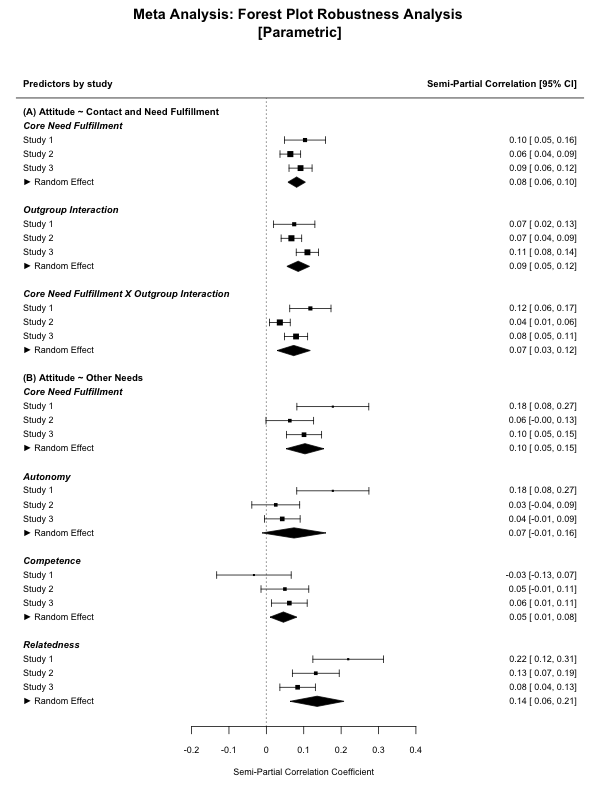
\includegraphics[width=\textwidth]{Figures/forestParametricRobustnessComb.png}
%   %\begin{subfigure}{\textwidth}
%   %  \caption{}
%   %  \centering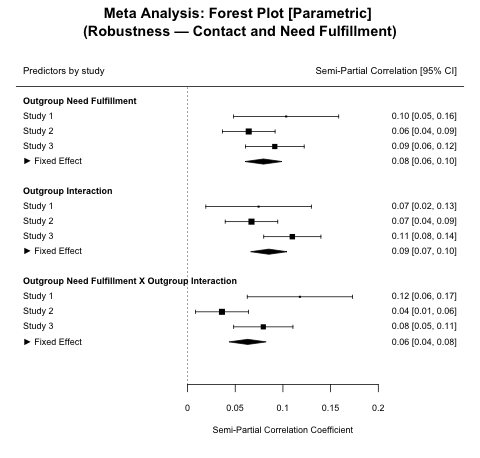
\includegraphics[width=0.65\textwidth]{Figures/forestParametricFERobustContact.png}
%   %\end{subfigure}
%   %\begin{subfigure}{\textwidth}
%   %  \caption{}
%   %  \centering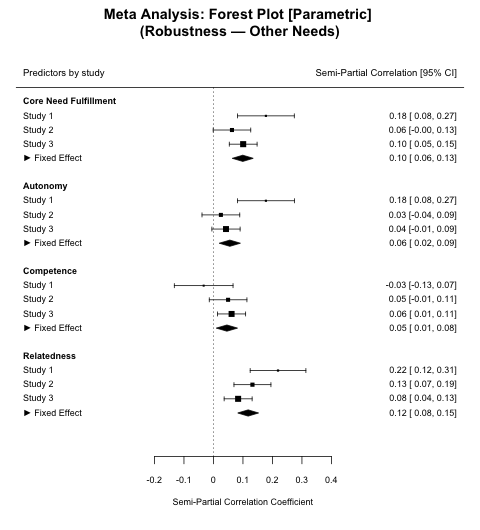
\includegraphics[width=0.65\textwidth]{Figures/forestParametricFERobustSDT.png}
%   %\end{subfigure}
%   \caption*{Note: \\
%   (a) Need Fulfillment and Intergroup Contact predicting Outgroup Attitudes (full sample).\\
%   (b) Core Need Fulfillment predicting Outgroup Attitudes while controlling for self-determination theory needs (intergroup contact sample).\\
%   General: Random effects meta-analytic results are presented for completeness.}
% \end{figure}


\end{document}
